\documentclass{article}
\usepackage{graphicx} % Required for inserting images
\usepackage{hyperref} % For clickable links
\usepackage{fancyhdr}  % For customizing the header and footer
% \usepackage{caption}
\usepackage{xcolor}         % For setting colors

% Customize hyperlink appearance
\hypersetup{
    colorlinks=true,        % Disable the boxes around links
    linkcolor=blue,         % Color for normal internal links
    urlcolor=blue,          % Color for external URLs
    citecolor=blue,         % Color for citations (if needed)
    filecolor=blue,         % Color for file links
    linkbordercolor=white,  % Hide the box around internal links (box is invisible)
    pdfborder={0 0 0},      % Remove the border around links
    footnotecolor=gray      % Color for footnote links
}

% Footnote link customization
\renewcommand\thefootnote{\textcolor{gray}{\arabic{footnote}}}  % Make footnote numbers gray


\title{Setting Up Controlbook Code and Python Environment for ME EN 431 / EC EN 483}
\author{Christian Hales, TA}
\date{Fall 2024}

\pagestyle{fancy}
\fancyfoot[C]{}  % Clear default center footer
\fancyfoot[L]{}  % Clear default left footer
\fancyfoot[R]{\hyperref[toc]{\textcolor{blue}{Table of Contents}}} % Right footer with link

\begin{document}

\maketitle
% Table of Contents Section
\section*{Table of Contents}
\label{toc}
\tableofcontents

\newpage

\section{Introduction}

This document explains how to set up your environment for the ME 431 / ECE 483 course.

These instructions are created by Christian Hales by combining his own instructions on virtual environments and Git upstream branches with Dr. Killpack's general instructions on how to use the controlbook code, as well as 2022 TA Carson Moon's instructions on general setup for creating a private copy of a public repository.

\section{Getting Started}

\subsection{Prerequisites}
Before setting up your environment locally, you need to install the following:

\begin{itemize}
    \item \textbf{Python}: You can download and install it from \href{https://www.python.org/downloads/}{python.org}.
    \item \textbf{Git}: Download and install it from \href{https://git-scm.com/downloads}{git-scm.com}.
    \item \textbf{VS Code}: Download and install it from \href{https://visualstudio.microsoft.com/downloads/}{Microsoft's website}.
\end{itemize}

\subsection{Setting Up VS Code}
\begin{center}
    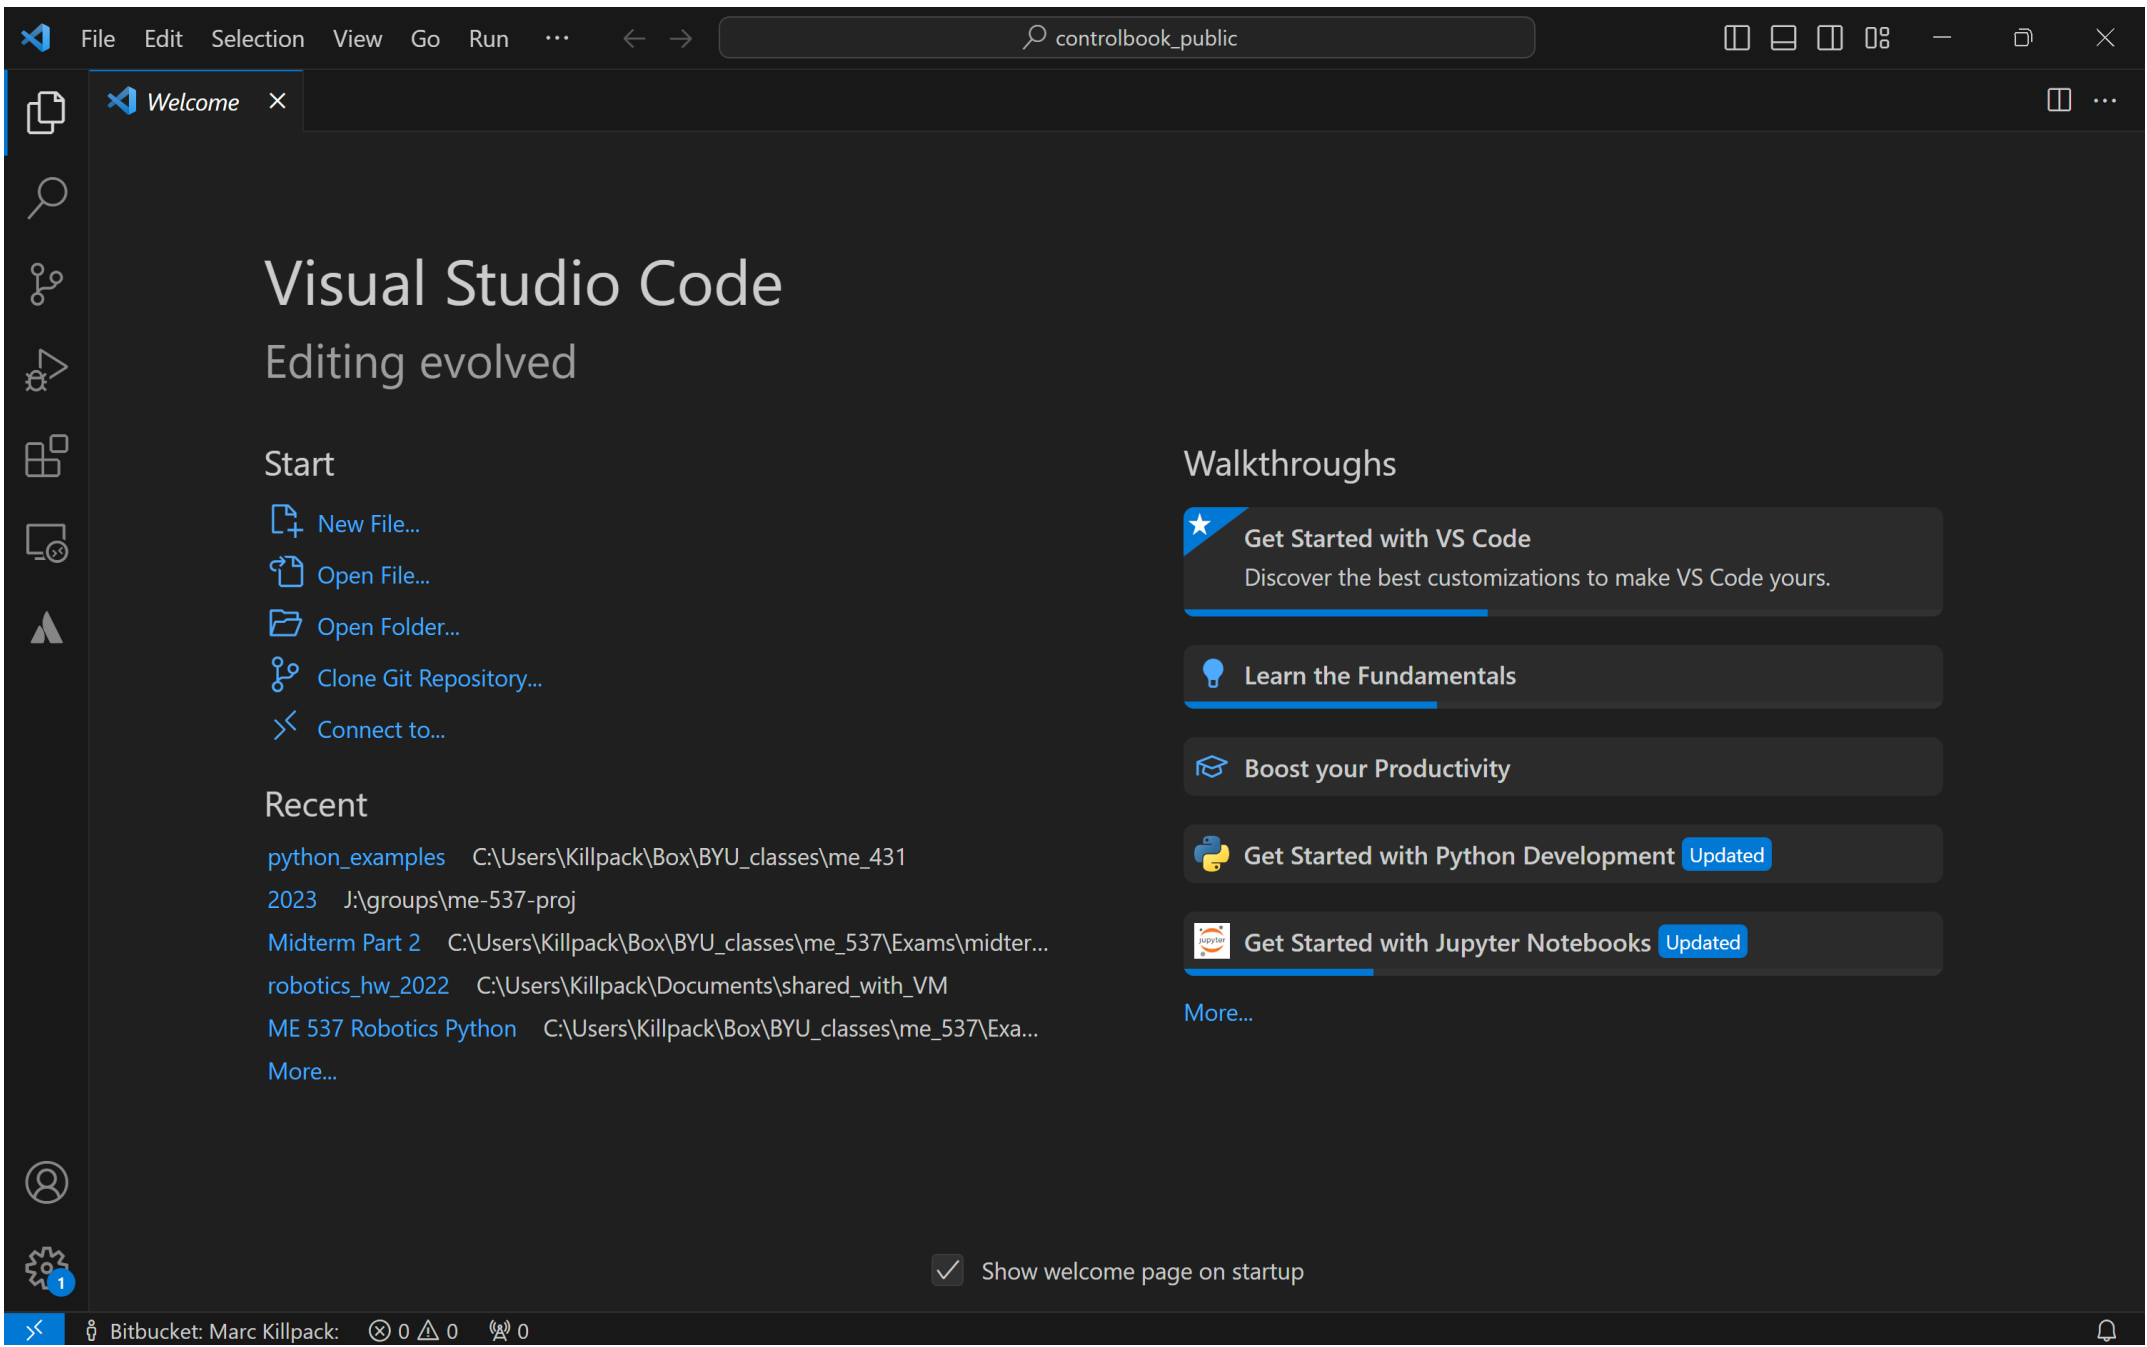
\includegraphics[width=\linewidth]{pic1-vsCodestarter.png} % Placeholder for the image
    \captionof{figure}{Visual Studios Home page}
\end{center}
Once you have installed VS Code, you need to install helpful extensions. Follow these steps:

\begin{enumerate}
    \item Click on the Extensions button in the sidebar.
    \item Search for ``Python'' and install the Python extension by Microsoft.
\end{enumerate}


\begin{center}
    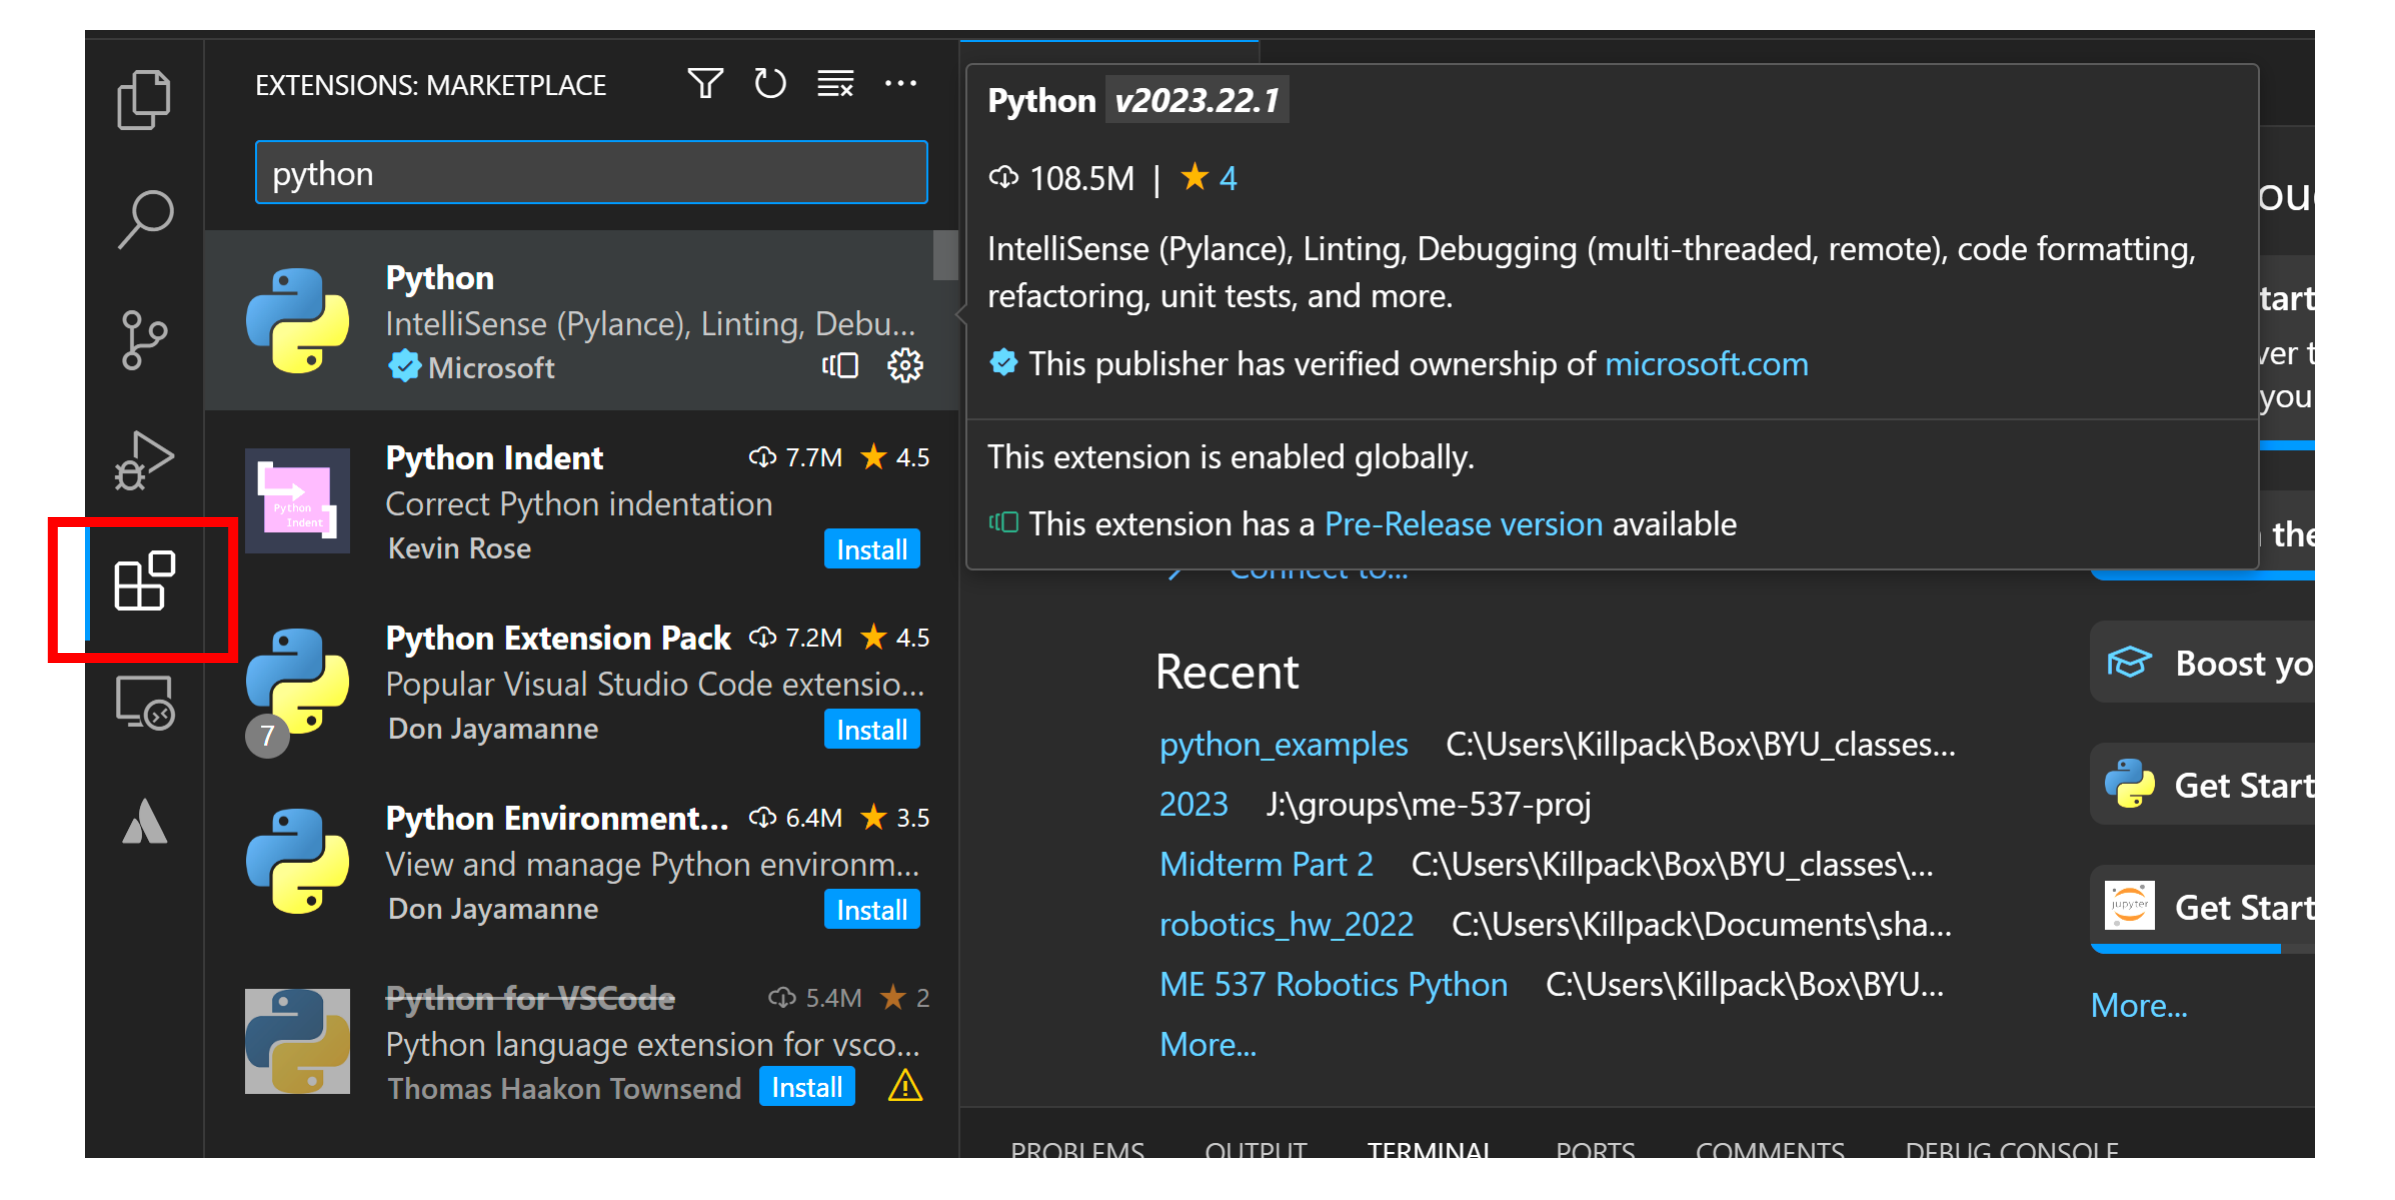
\includegraphics[width=\linewidth]{pic2-vsCodeExtensions.png}
    \captionof{Installing Python Extension}
\end{center}

\subsection{Making a Private Clone of the Public Repo}
To avoid sharing code and keeping with BYU Honor Code, you will want to create a private clone of the public repository.
\newline
\newline
Follow these steps:

\subsubsection{Creating a Private Repo}
\begin{enumerate}
    \item Go to \href{https://github.com/new}{GitHub's new repository page}.
    \item Name your new repository (e.g., \texttt{control\_systems}).
    \item Ensure it is set to ``Private'' and create the repository.
\end{enumerate}

\subsubsection{Cloning the Repo and Connecting to the Upstream Remote}
In your terminal:

\begin{enumerate}
    \item Clone your new private repository using the HTTPS URL provided.
     
\begin{center}
    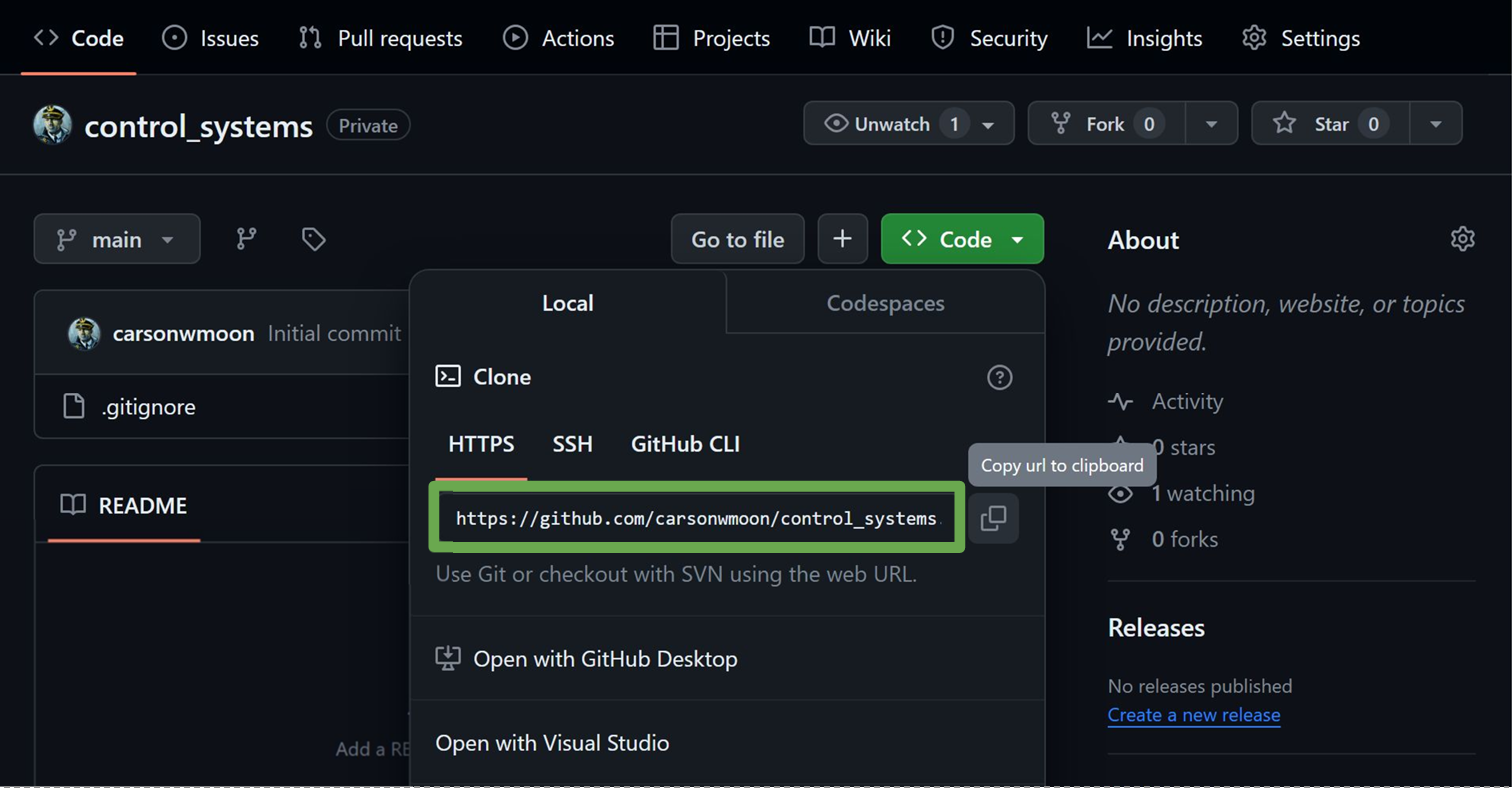
\includegraphics[width=\linewidth]{pic7b-clone.png} % Placeholder for the image
    \captionof{Grabbing the private repo's link}
\end{center}
\begin{center}
    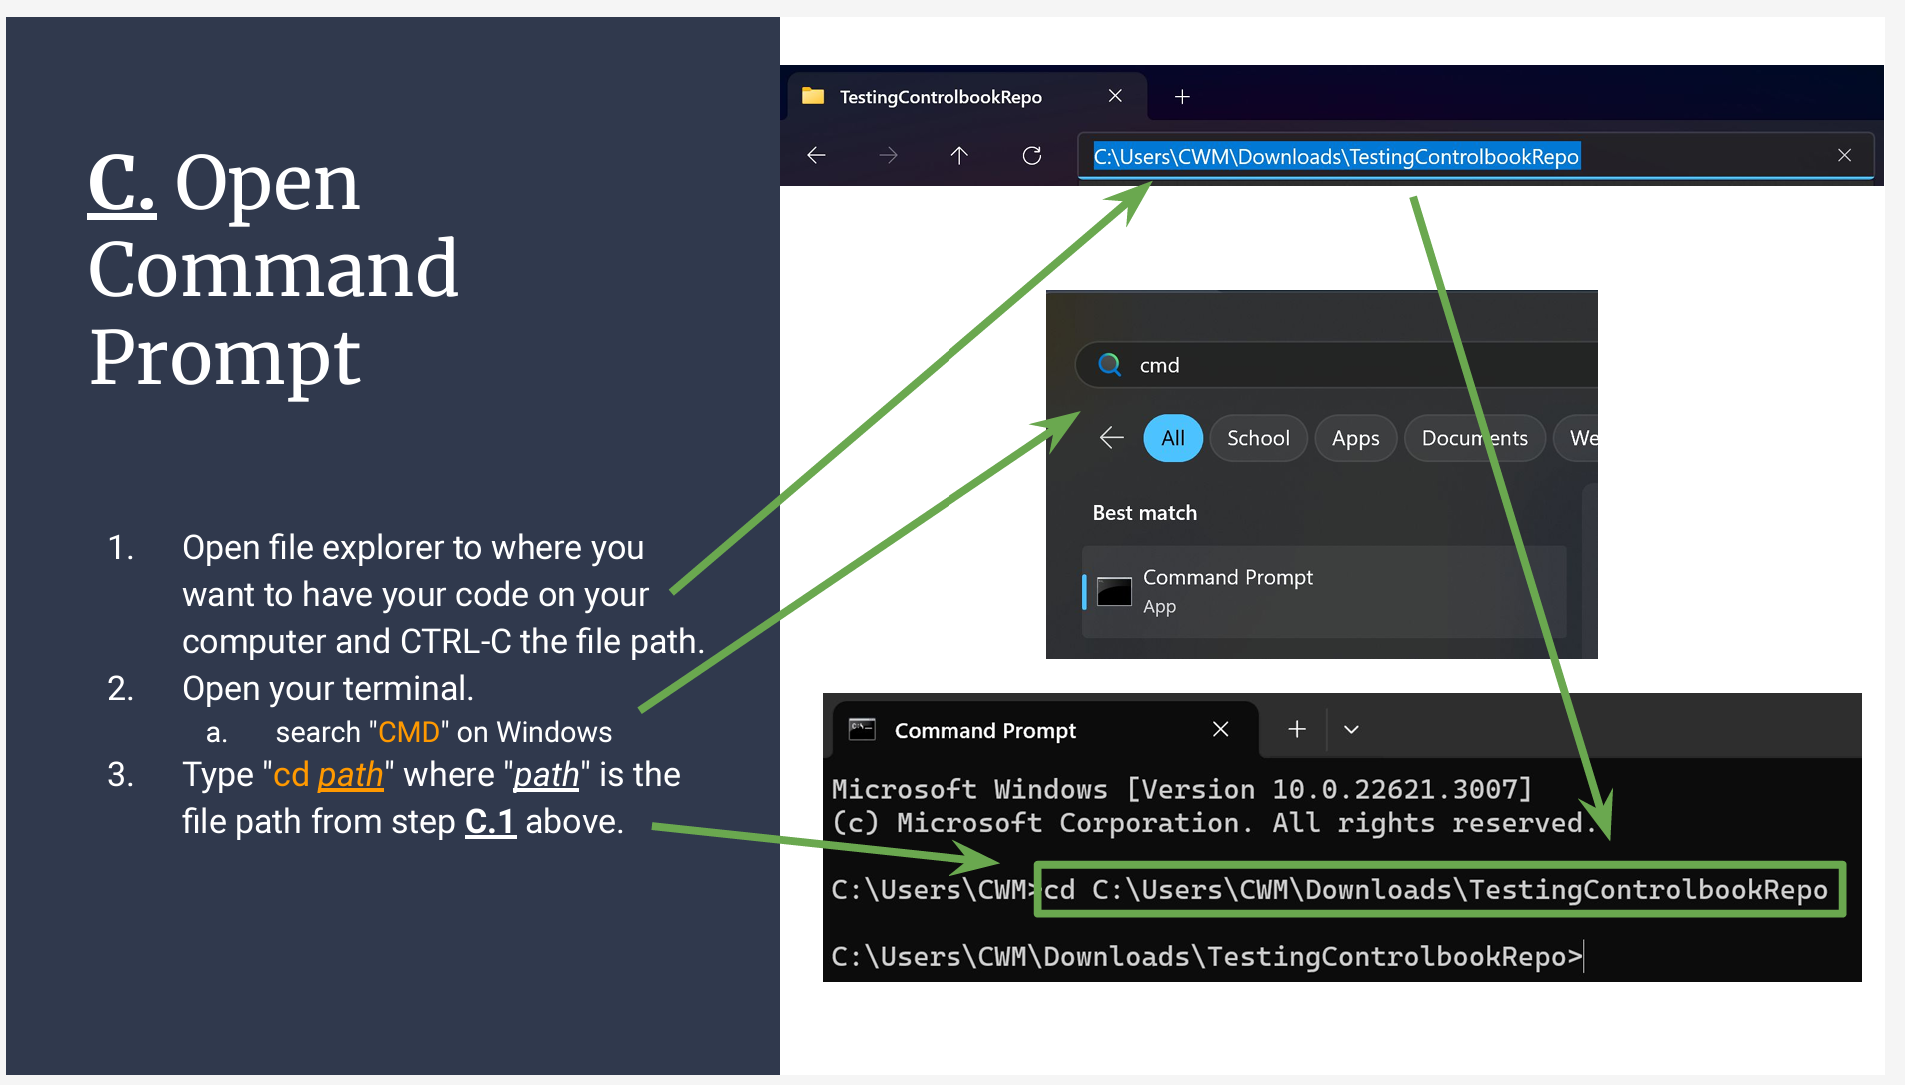
\includegraphics[width=\linewidth]{pic7d-opening-terminal.png} % Placeholder for the image
    \captionof{Using command line -- Windows Powershell is used, but any shell can be used.\footnote{A shell refers to Git/Linux Bash, Powershell, Mamba, etc. Note that Git must be installed for Powershell to run Git commands. }\footnote{Also note that in VSCode, any of these shells can be opened by pressing Ctrl-`, where "`" is a tickmark found to the left of the number-1 button.}}
\end{center}
    \item Then \texttt{cd} into the repository.
    \item Connect to the public Controlbook repo by running:
\begin{verbatim}
git remote add upstream https://github.com/byu-controlbook/controlbook_public.git
\end{verbatim}
    \item Type \texttt{git remote -v} to check your connection to both repositories.
\end{enumerate}

 
\begin{center}
    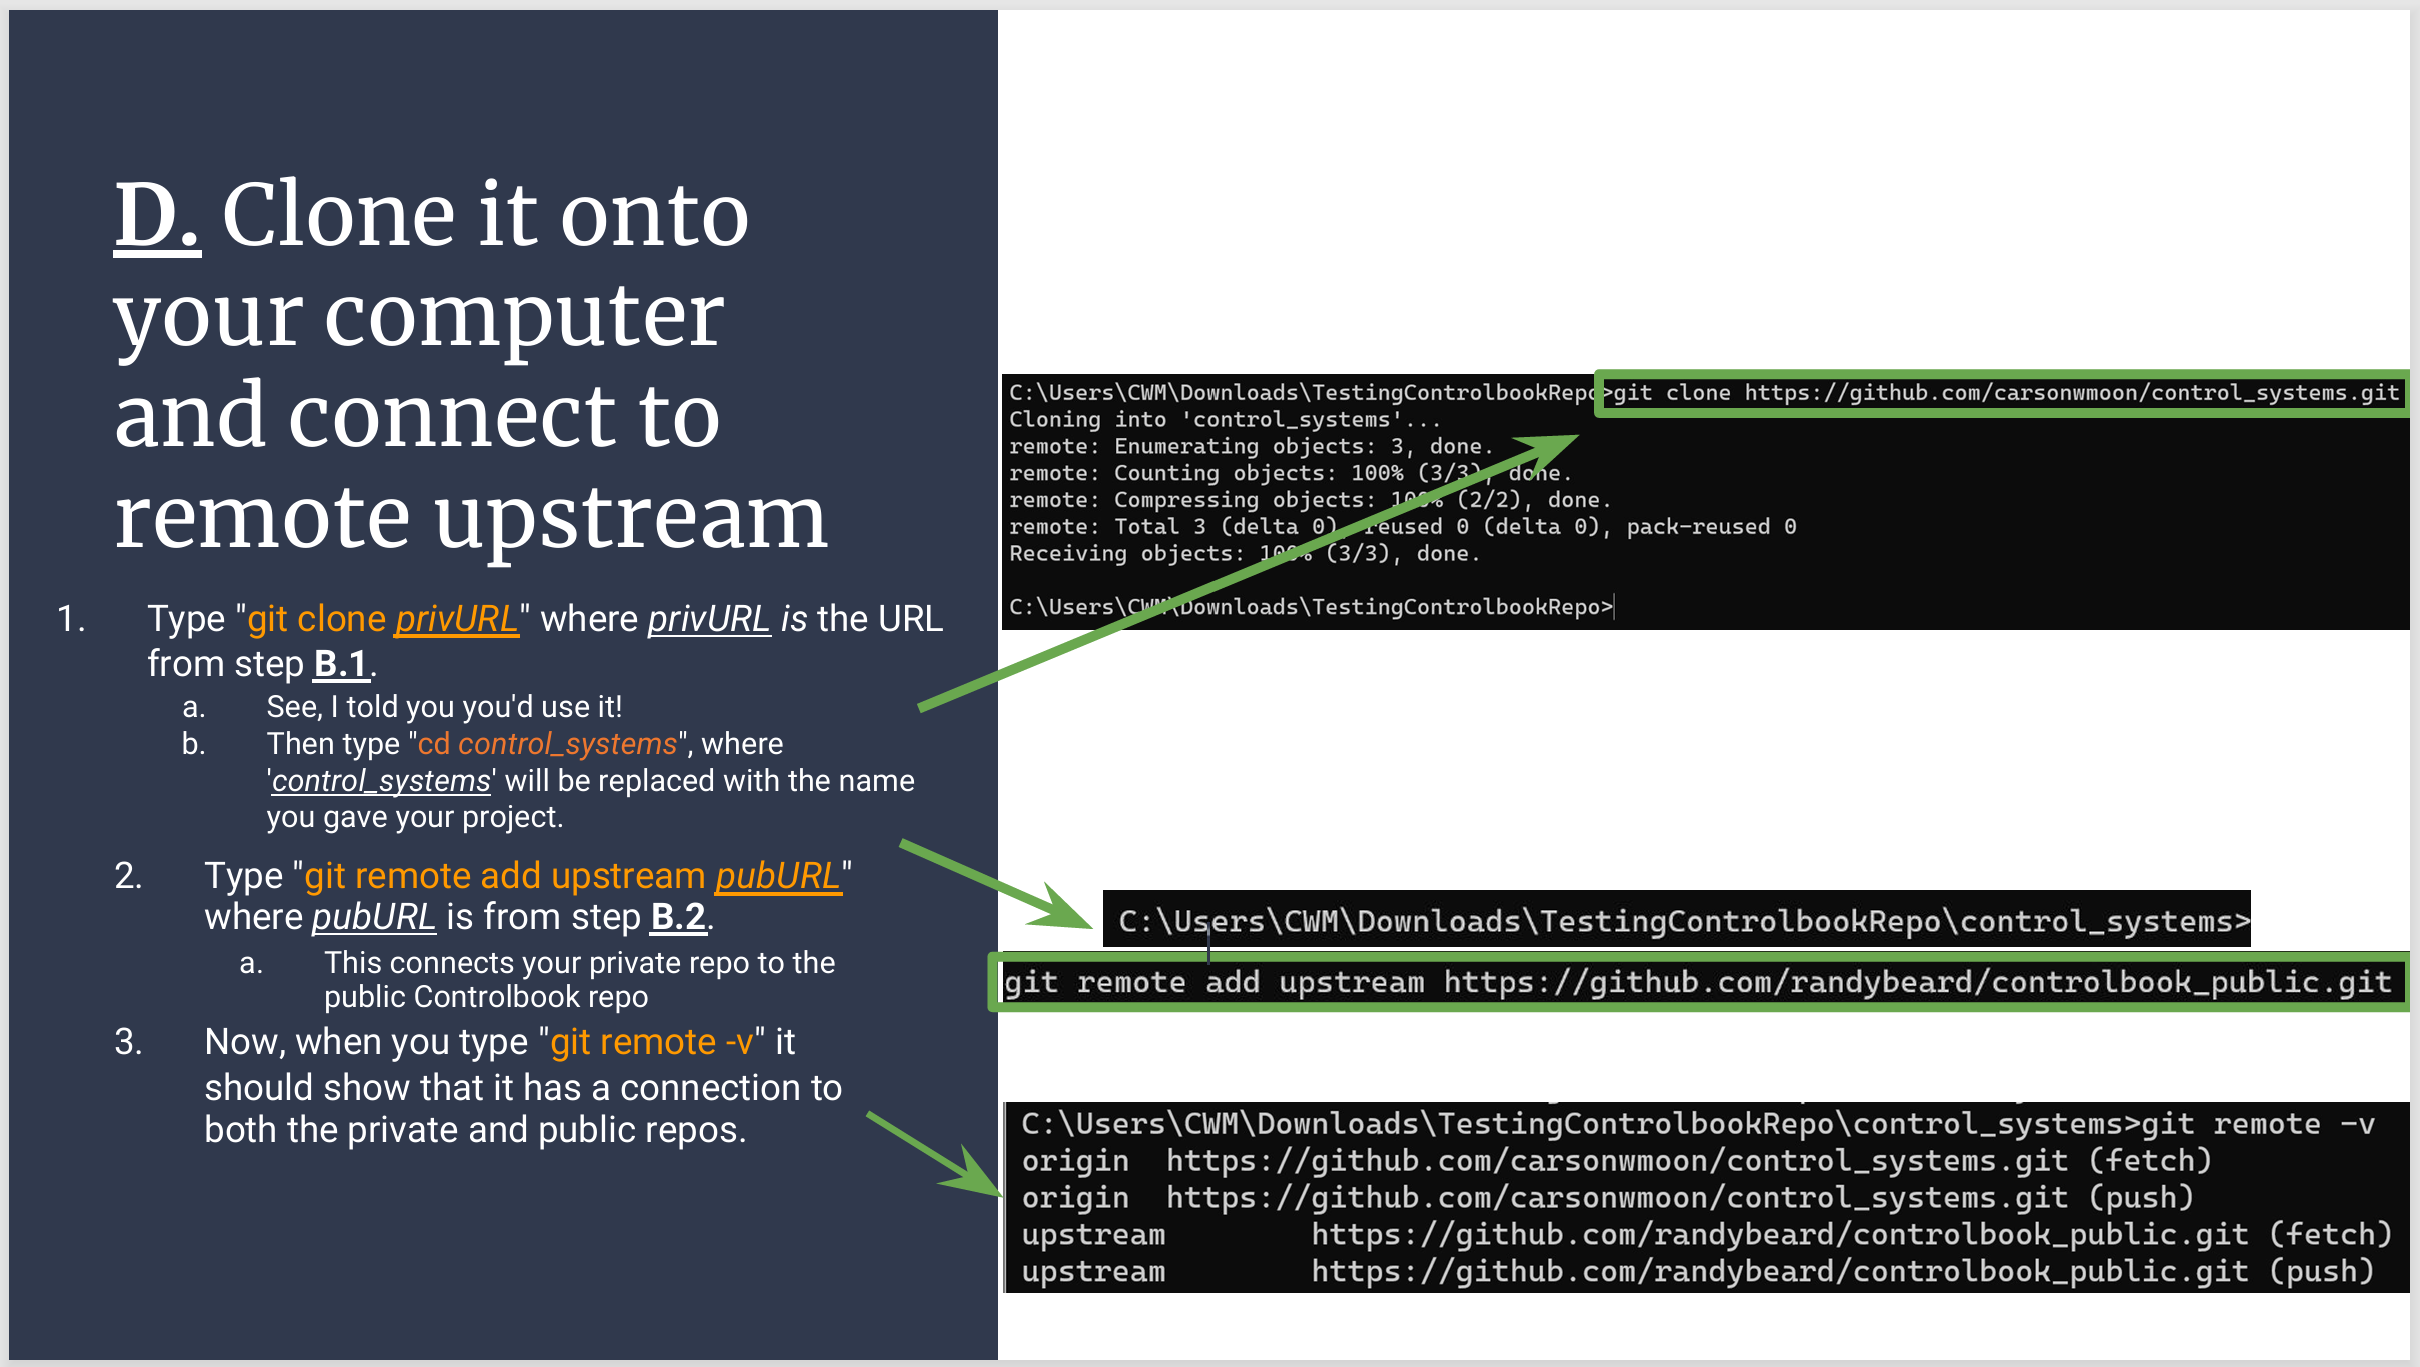
\includegraphics[width=\linewidth]{pic7e2.png} % Placeholder for the image
    \captionof{Previous two steps using Carson's slides}
\end{center}

\subsubsection{Fetching and Merging from the Public Repo}
\label{copy-repo}
To get the first copy of the public repository, and to fetch changes from the public repo in the future (do not copy verbatim):

\begin{verbatim}
git fetch upstream <current Branch>
git merge --allow-unrelated-histories upstream/<current Branch>
git push
\end{verbatim}



In the above \texttt{Git} commands, \texttt{<current Branch>} is this semester's branch of code that will be used.\footnote{Look to the TAs for which branch of the code to use. In Fall2024, the \texttt{2024Winter} branch was used. Often in industry, the main branch that runs all of the code is the \texttt{master} or \texttt{main} branch. Development would then be done on separate branches which are then merged into the \texttt{master} or \texttt{main} branch.} 

\begin{center}
    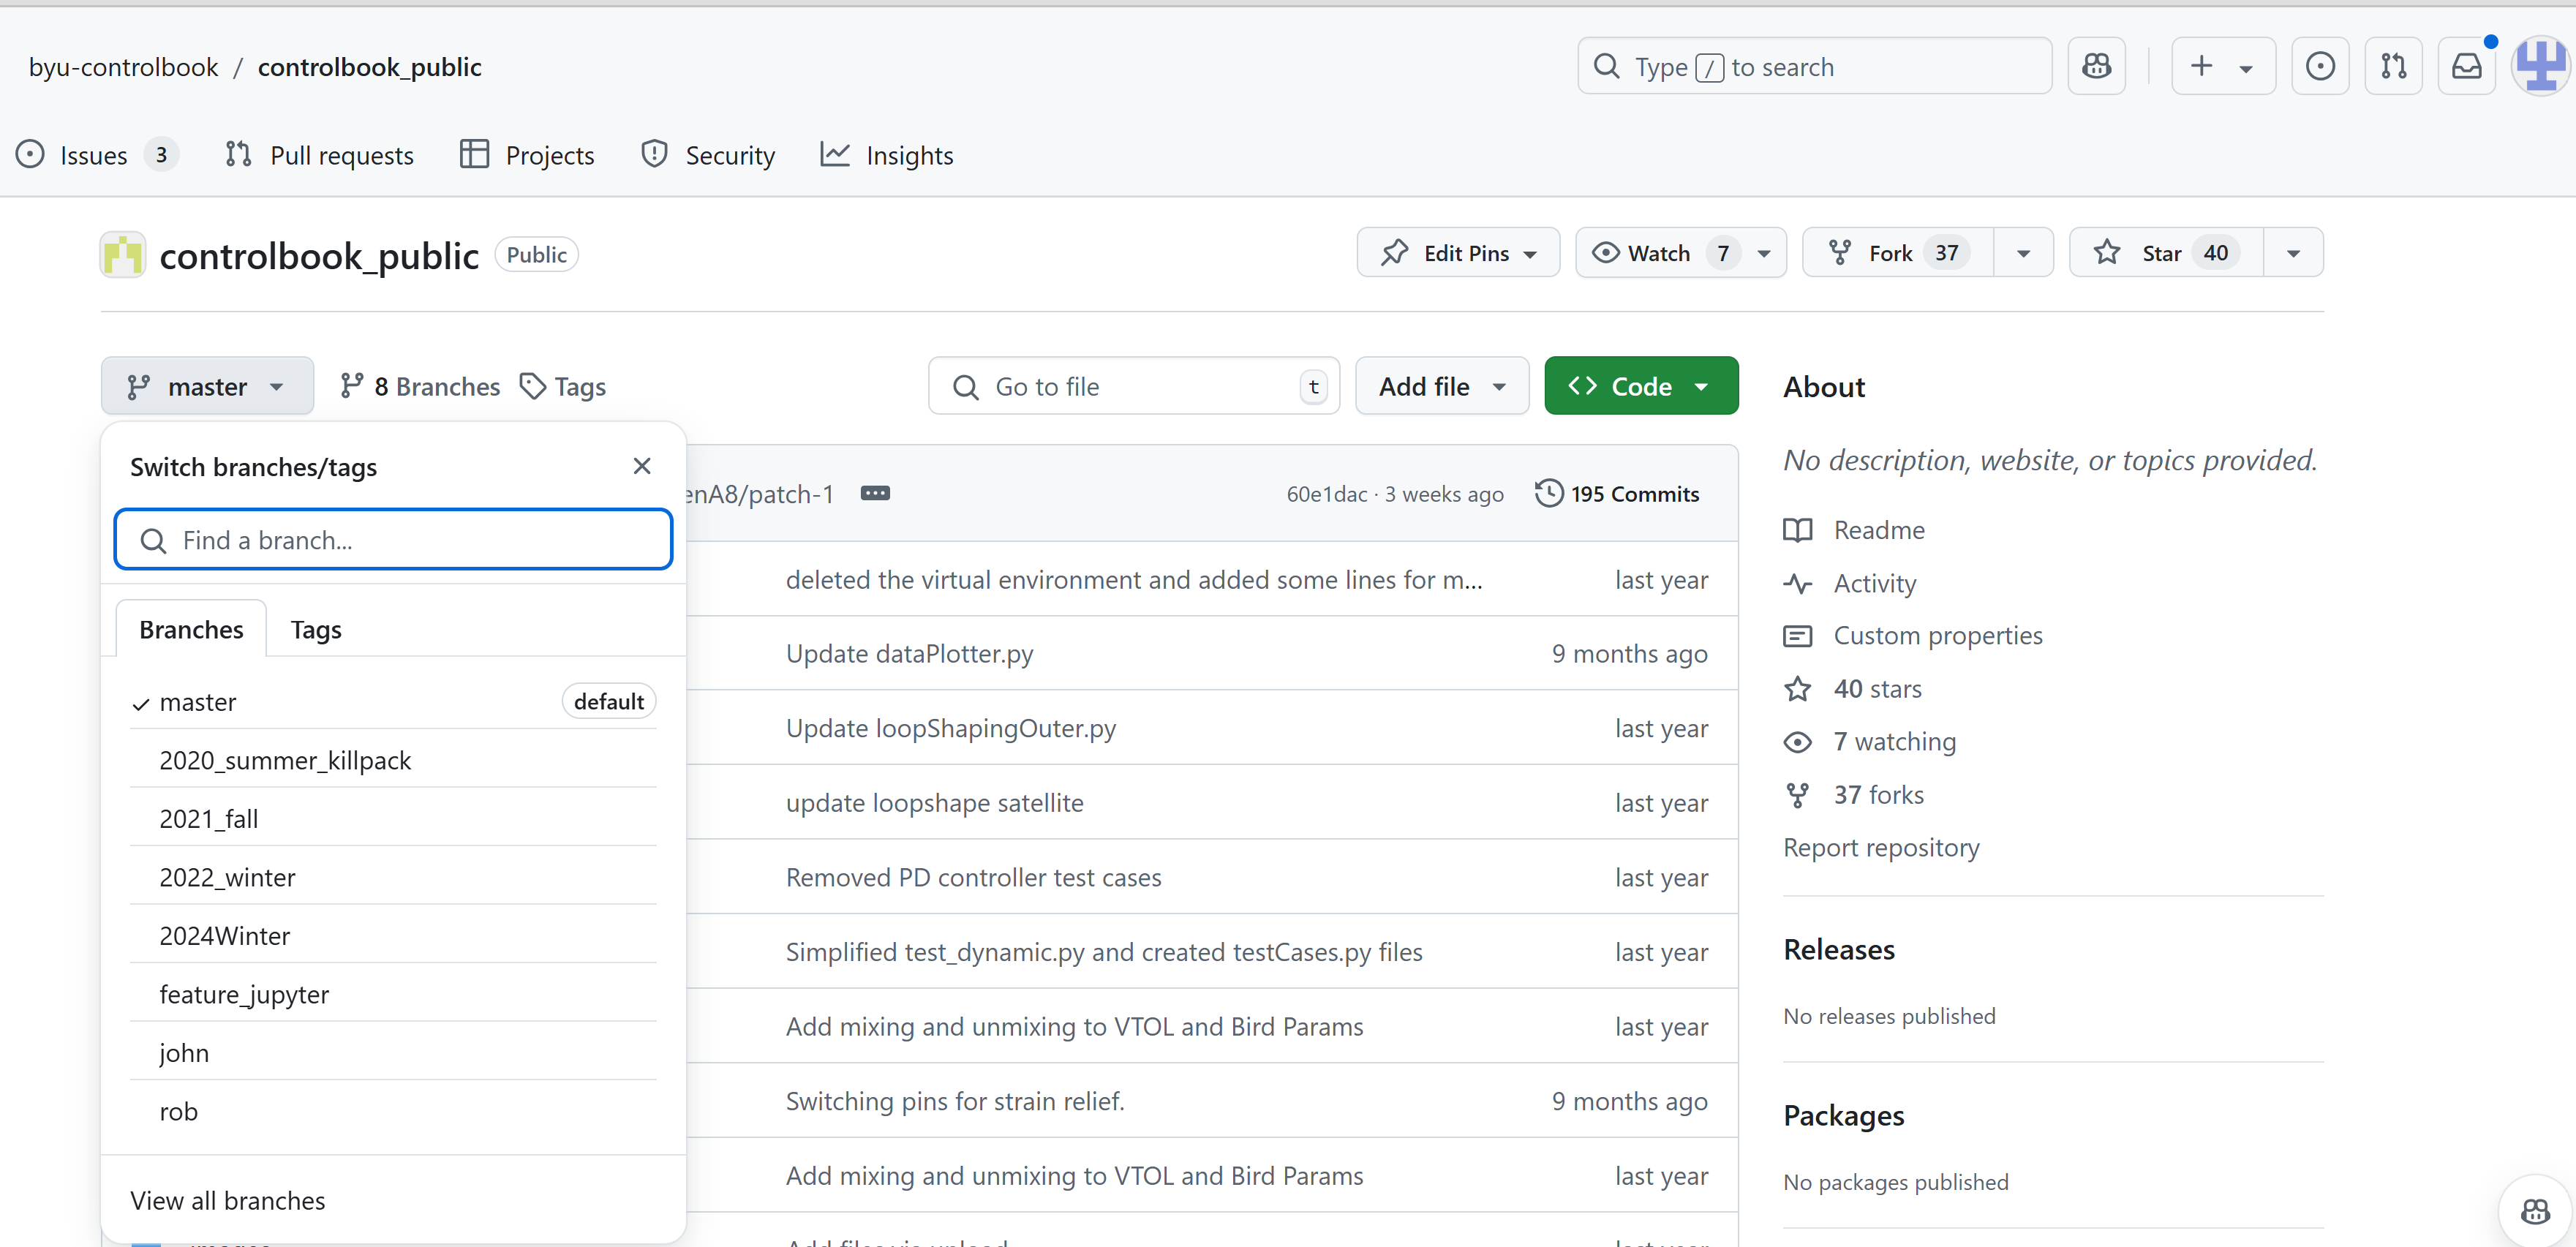
\includegraphics[width=\linewidth]{pic7f-differentBranches.png} 
    \captionof{Examples of the different branches}
\end{center}

\section{Setting Up Python Environment}

\noindent Below are two different methods for setting up your Python environment for this course:

\begin{itemize}
    \item \textbf{Option A:} Install necessary Python libraries directly on your local machine.
    \item \textbf{Option B:} Set up a virtual environment to manage dependencies.
\end{itemize}

\textbf{DO NOT CHOOSE Option A.}

\subsection{Why Virtual environments}
A simple web search or AI search will provide dozens of reasons why virtual environments are important. Here are two reasons that are relevant to the Controls class:
\begin{itemize}
    \item \textbf{Easier Collaboration and Debugging}: When working in a team (or amongst multiple students using the same class code), using virtual environments helps ensure that everyone has the same environment setup.
    \item \textbf{Dependency Isolation}: Each Python project may rely on different versions of the same libraries. Installing these globally on your system can lead to conflicts between projects.
\end{itemize}



\subsection{Setting \texttt{venv}}
More than a dozen different industry-standard options for virtual environments are available.\footnote{See \hyperref[appendix-a]{Appendix A} for more information.} In this class, virtual environments are installed directly in VSCode by using VSCode's built-in features, which implement Option 1 in \hyperref[appendix-a]{Appendix A} (the \textit{venv} method), as explained in  \href{https://code.visualstudio.com/docs/python/environments#_creating-environments}{this link}. Please use that link to set up the virtual environment in VSCode.

\subsection{Activating \texttt{venv}}

After setting up a virtual environment as described in the \href{https://code.visualstudio.com/docs/python/environments#_creating-environments}{VS Code documentation}, you will need to activate it in your terminal. The steps for creating and activating the environment are slightly different depending on whether you're using a Windows machine or a Linux/macOS machine. \textbf{You will need to do this each time you open a terminal in the project.} \footnote{A new virtual environemnt can be made by calling \texttt{python -m venv .venv} (or \texttt{python3} for MacOS/Linux). Note that \texttt{.venv} is a common user-assigned name, but any name for the virtual environment could be chosen. If one deisred, multiple environments could be made.}

\subsubsection{Windows Instructions}
On Windows, after creating the virtual environment, you activate it by running the following command in the terminal:

\begin{verbatim}
.\.venv\Scripts\activate
\end{verbatim}

\subsubsection{Linux/macOS Instructions}

\begin{verbatim}
source .venv/bin/activate
\end{verbatim}

\begin{center}
    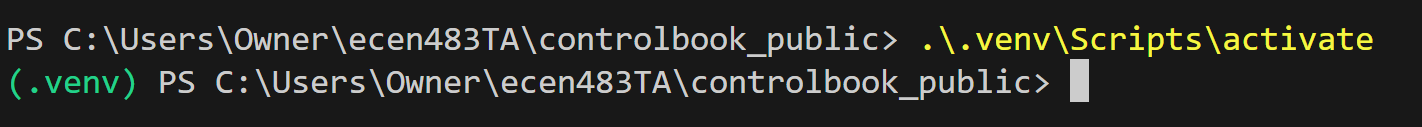
\includegraphics[width=\linewidth]{pic7g-venv.png} 
    \captionof{Activating venv on CLI (Command Line Interface\footnote{ The venv should already be configured with VSCode. This step is only necessary for installation of libraries. While venv CLI can indeed run python files, this pdf will teach you how to run files in venv through VSCode's GUI.})}
\end{center}

Once activated, you can move on to the next step.

\subsection{Installing Required Libraries}

Install libraries in the virtual environment by running:

\begin{verbatim}
pip3 install -r requirements.txt
\end{verbatim}
If, for some reason, there is no \texttt{requirements.txt} in the project\footnote{As of October 2024, the only branch of the project to have this was the \textbf{2024Winter} branch. 
}, one can get started in the project by looking up how to install \texttt{numpy}, \texttt{control} and \texttt{matplotlib} libraries on your specific shell\footnote{A shell refers to \texttt{Git/Linux Bash}, \texttt{Powershell}, \texttt{Mamba}, etc.}. Other libraries can be installed as the need arises.

\textbf{For TAs:} If a \texttt{requirements.txt} or any other big change is needed, it be created by a Pull Request (\texttt{PR}). See \hyperref[appendix-b]{Appendix B} for more information.

\section{Updating Personal Repo}

\subsection{General Process for Personal Repo}
After making changes to your project files, follow the process to add, commit, and push your changes to your Git repository.

\textbf{NOTE: } If you are looking for a simple list of bash commands to follow, go to \hyperref[summaryGit]{the commands found in Summary below}.
\begin{enumerate}
    \item \textbf{Stage the changes}: The first step is to tell Git which files have changed and need to be tracked. You can stage all files or specific files using the following commands:

    \begin{verbatim}
    # To stage all changed files (includes newly created files):
    git add .
    
    # Alternatively, to stage a specific file:
    git add <filename>
    \end{verbatim}

    \item \textbf{Commit the changes}: Once the files are staged, you need to commit the changes. Committing records the changes to the repository and allows you to add a message explaining the changes you made:

    \begin{verbatim}
    # To commit all staged files:
    git commit -m "Descriptive message about the changes"

    # Alternatively, to commit and stage all files that have been staged before
    # (This does NOT include new, untracked files)
    # (This CAN replace "git add" if there are no newly created files):
    git commit -am "Descriptive message about the changes"
    \end{verbatim}

    
    A good commit message describes what changes were made and why they were necessary, helping track the project's history


    \item \textbf{Push the changes}: The final step is to push your committed changes to your remote repository (e.g., on GitHub). This updates the remote repository with the latest code from your local machine:

    \begin{verbatim}
    # Option 1: Push to specific branch
    git push origin <branchname>
    # Option 2: Push all changes generally
    git push
    \end{verbatim}

    Replace \texttt{branchname} with the name of the branch you are working on (e.g., `main`, `development`, etc.). This ensures your changes are saved and accessible from other locations.
    \subsubsection{Summary of Updating Personal Project Repo}
    
    \label{summaryGit}

    In summary, a good general process is:
    \begin{verbatim}
    git add .
    git commit -am "Write a unique message here"
    git push
    \end{verbatim}
\end{enumerate}

\subsection{Grabbing Changes from Controlbook}
Occasionally, changes will be made to the class code, which will require grabbing the changes from the public repo. Follow the steps in \hyperref[copy-repo]{Fetching and Merging from the Public Repo}  to do so.\footnote{In group projects, best policy is to grab all changes to repositories and group items. This includes performing \texttt{git pull} at the start of every day.}


\subsection{Pull Requesting Controlbook}
\textbf{For TAs:} You will not push changes to controlbook, but if changes do need to be made, a separate fork can be made, updating the specific problem on your fork and submitting a request to the project with the specific changes. See \hyperref[appendix-b]{Appendix B} for more details on the subject. 

\section{Test Matplotlib}

Now that the environment is set up, you should check to make sure your computer creates good plots. Navigate to an example file by clicking the button in \textcolor{red}{red} shown in the image below, and then selecting a file such as:

\begin{quote}
\texttt{A\_arm->python->hw03\_armSim.py}
\end{quote}


\begin{center}
    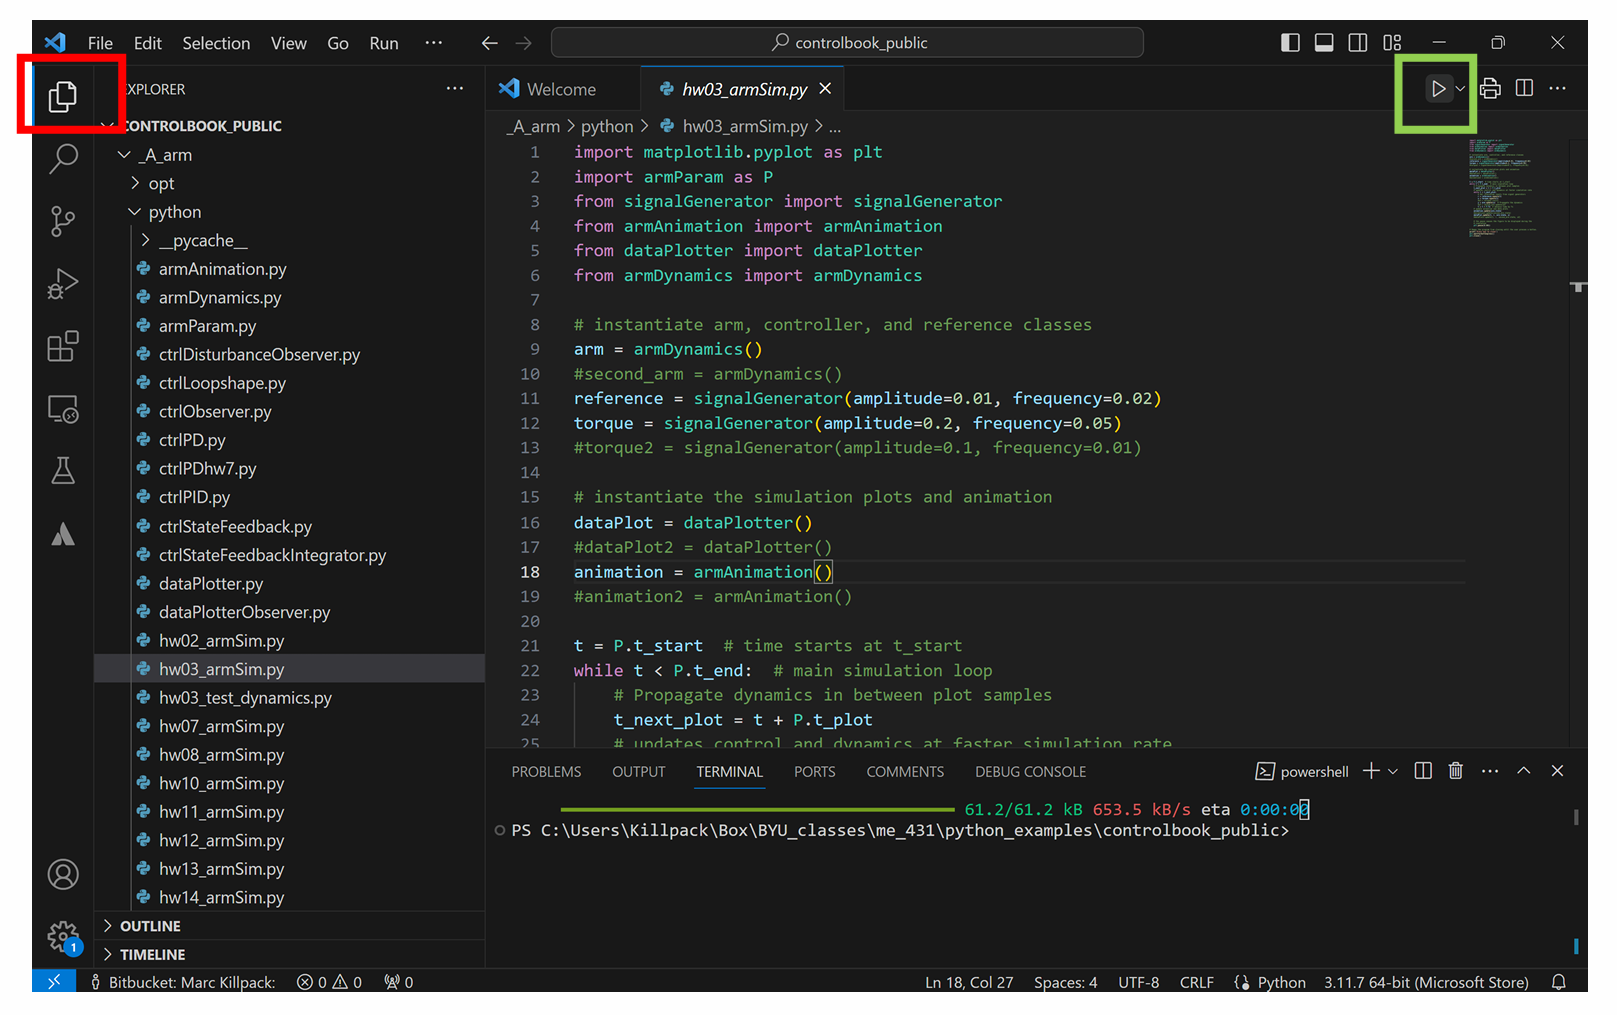
\includegraphics[width=\linewidth]{pic8-red-green.png} 
    \captionof{Files in Project}
\end{center}

After selecting this file, you can run the code by pushing the button in \textcolor{green}{green} shown above.


If the visualization blinks and doesn’t render properly (most likely a problem on Windows computers), you can change what graphics library is being used to render the plots. 

Do this by opening the relevant \_\_\_\_Animation.py file (which is case-study dependent) as shown below. Then uncomment any \texttt{matplotlib.use} line. For example:

\begin{quote}
\texttt{matplotlib.use(‘tkagg’)}
\end{quote}

\begin{center}
    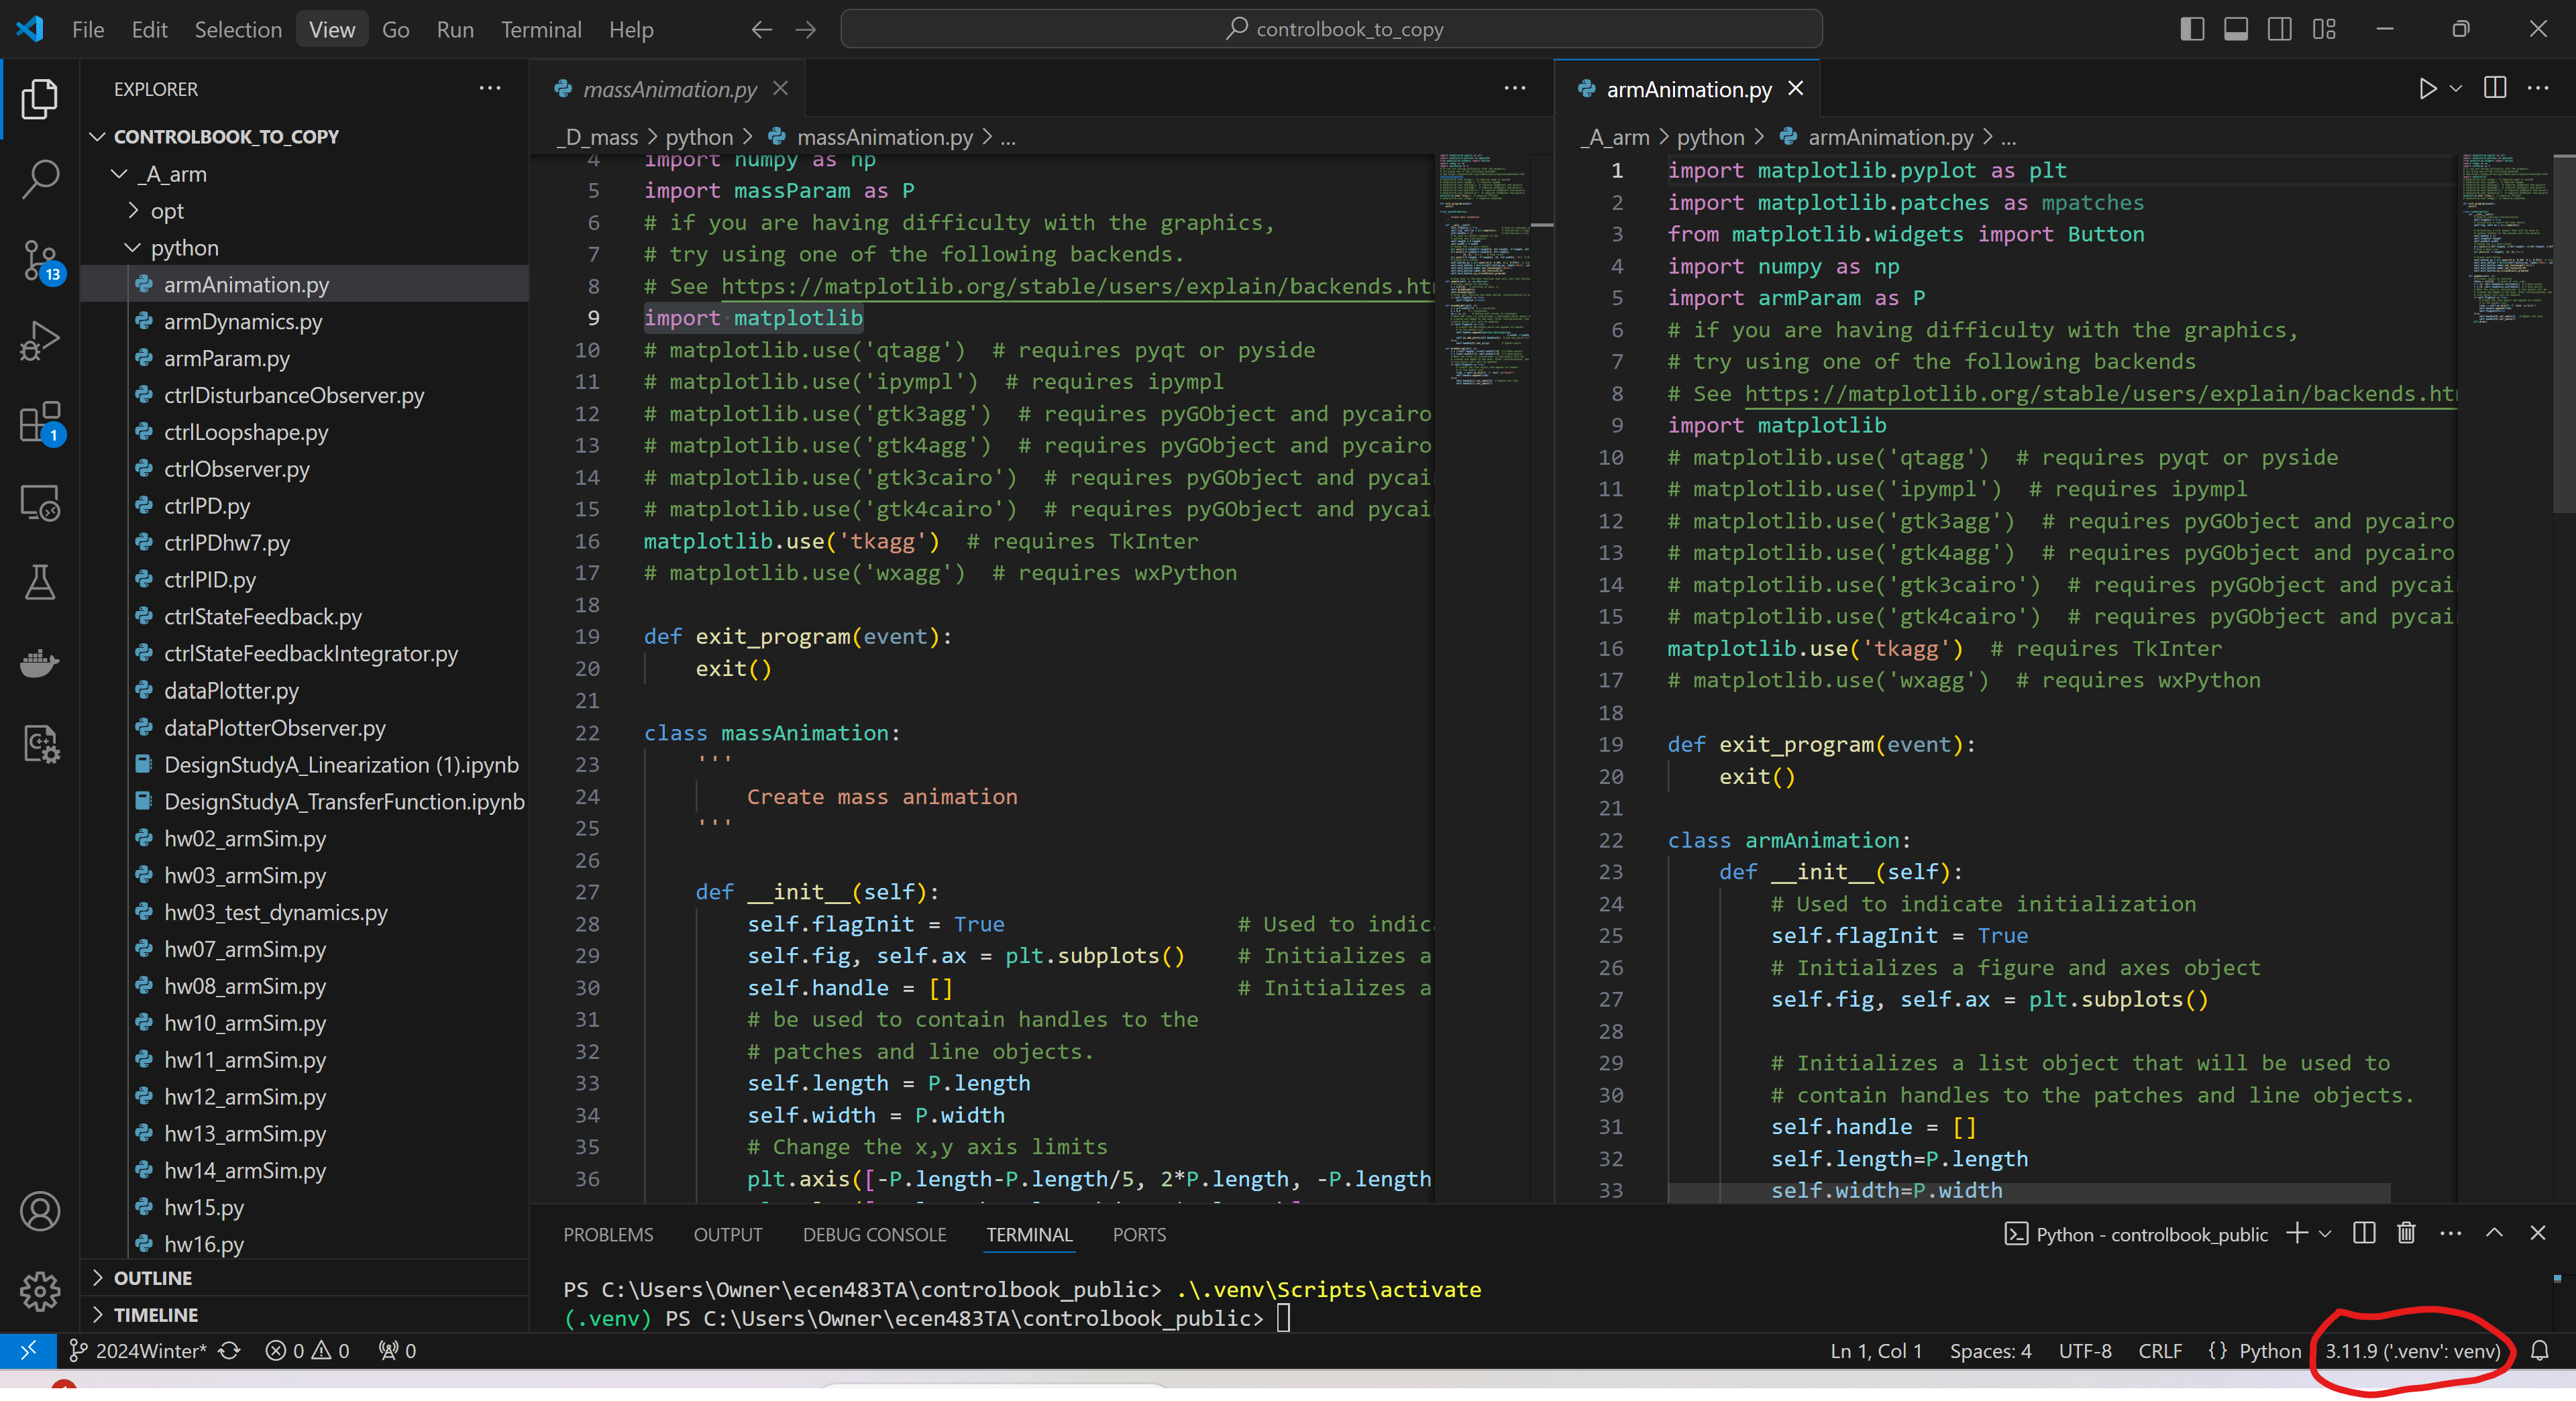
\includegraphics[width=\linewidth]{pic8-final.png} 
    \captionof{Matplotlib files in Cases A and D. \footnote{Note also the Virtual Environment kernel circled in the bottom right-hand corner. This shows that the environment is properly set up.}}
\end{center}

 It should make a big difference. After uncommenting that line, navigate back to the main file to run it. You will have to do this on every case study, unfortunately, but only the first time.

 If you still run into errors, it may be helpful to directly add the following to the top of your simulation file:

 \begin{verbatim}
     import matplotlib
     matplotlib.use(‘tkagg’)
 \end{verbatim}




\section{Conclusion}
This document covered the three main methods for setting up your environment for ME EN 431 / EC EN 483: installing libraries and Python IDE on your local machine, setting up a virtual environment, and configuring Matplotlib. Additionally, instructions for making a private clone of the public repository were provided.

\newpage

\appendix

\section{Other Virtual Environments}
\label{appendix-a}
Virtual environments in Python are essential for managing dependencies and ensuring that different projects can use different versions of the same libraries without conflicts. Below is a list of common methods for creating and managing virtual environments, each suited to different use cases:

\subsection{1. \texttt{venv} (Built-in Python Virtual Environment)}
The \texttt{venv} module is a built-in tool in Python (from version 3.3 and up) that allows for the creation of lightweight virtual environments. It is a simple and effective way to isolate dependencies for each project.

\begin{itemize}
    \item \textbf{Usage}: 
    \begin{verbatim}
    python -m venv <env_name>
    source <env_name>/bin/activate  # On Linux/macOS
    .\<env_name>\Scripts\activate  # On Windows
    \end{verbatim}
    \item \textbf{Pros}: Built-in, lightweight, and easy to use.
    \item \textbf{Cons}: Basic functionality, lacks some advanced features like dependency management found in other tools.
\end{itemize}

\subsection{2. \texttt{conda} (Environment and Package Manager)}
\texttt{conda} is a powerful environment and package manager that is popular in the data science community. It manages both Python and non-Python dependencies and can create isolated environments for different projects.

\begin{itemize}
    \item \textbf{Usage}: 
    \begin{verbatim}
    conda create --name <env_name> python=3.x
    conda activate <env_name>
    \end{verbatim}
    \item \textbf{Pros}: Excellent for managing complex dependencies, especially useful in data science projects. Works across programming languages.
    \item \textbf{Cons}: Environments tend to be larger in size, and it requires \texttt{conda} (or Anaconda/Miniconda) installation.
\end{itemize}

\subsection{3. \texttt{mamba} }
\texttt{mamba} (Fast Conda Alternative) is a reimplementation of \texttt{conda} in C++ that focuses on speed. It significantly reduces the time needed for environment creation and dependency resolution while maintaining compatibility with \texttt{conda}.

\begin{itemize}
    \item \textbf{Usage}: 
    \begin{verbatim}
    mamba create --name <env_name> python=3.x
    mamba activate <env_name>
    \end{verbatim}
    \item \textbf{Pros}: Much faster than \texttt{conda}, especially with large environments and complex dependencies.
    \item \textbf{Cons}: Requires \texttt{mamba} installation, but otherwise compatible with \texttt{conda}.
\end{itemize}

\subsection{4. \texttt{Docker} (Containerization Tool)}
While not strictly a virtual environment, \texttt{Docker} allows you to create isolated containers that can include the entire software stack (OS, libraries, dependencies). This makes it more powerful than just isolating Python dependencies.

\begin{itemize}
    \item \textbf{Usage}: 
    \begin{verbatim}
    docker run -it python:3.x bash
    \end{verbatim}
    \item \textbf{Pros}: Full isolation of the application, including system-level dependencies. Excellent for reproducibility and deployment.
    \item \textbf{Cons}: Requires knowledge of containerization, more overhead than typical virtual environments.
\end{itemize}

\subsection{5. \texttt{virtualenv}}
\texttt{virtualenv} is a widely-used tool for creating isolated Python environments. It predates \texttt{venv}, but offers more features and better support for older Python versions.

\begin{itemize}
    \item \textbf{Usage}: 
    \begin{verbatim}
    pip install virtualenv
    virtualenv <env_name>
    \end{verbatim}
    \item \textbf{Pros}: Supports both Python 2.x and 3.x, provides more features than \texttt{venv}.
    \item \textbf{Cons}: Requires installation, overlaps with \texttt{venv}.
\end{itemize}

\subsection{6. \texttt{pipenv}}
\texttt{pipenv} integrates environment creation with dependency management by using a \texttt{Pipfile} and \texttt{Pipfile.lock} for better reproducibility.

\begin{itemize}
    \item \textbf{Usage}: 
    \begin{verbatim}
    pip install pipenv
    pipenv install
    pipenv shell
    \end{verbatim}
    \item \textbf{Pros}: Combines virtual environments with dependency management, great for project reproducibility.
    \item \textbf{Cons}: Slower than \texttt{venv} or \texttt{virtualenv}, can be more complex.
\end{itemize}

\subsection{7. \texttt{poetry}}
\texttt{poetry} is a modern tool for dependency management and packaging in Python. It uses the \texttt{pyproject.toml} file for managing dependencies and packaging.

\begin{itemize}
    \item \textbf{Usage}: 
    \begin{verbatim}
    pip install poetry
    poetry install
    poetry shell
    \end{verbatim}
    \item \textbf{Pros}: Combines environment management, dependency resolution, and packaging in one tool.
    \item \textbf{Cons}: Heavier than \texttt{venv}, more complex for small projects.
\end{itemize}

\subsection{8. \texttt{pyenv} + \texttt{pyenv-virtualenv}}
\texttt{pyenv} allows for the management of multiple Python versions, while \texttt{pyenv-virtualenv} integrates virtual environments into this workflow.

\begin{itemize}
    \item \textbf{Usage}: 
    \begin{verbatim}
    pyenv install 3.x.x
    pyenv virtualenv 3.x.x <env_name>
    \end{verbatim}
    \item \textbf{Pros}: Easily switch between multiple Python versions, integrates well with virtual environments.
    \item \textbf{Cons}: Limited to Linux/macOS, more setup required.
\end{itemize}

\subsection{9. \texttt{tox}}
\texttt{tox} is a tool designed for automating testing across multiple Python environments. It is widely used in continuous integration (CI) pipelines.

\begin{itemize}
    \item \textbf{Usage}: 
    \begin{verbatim}
    pip install tox
    tox
    \end{verbatim}
    \item \textbf{Pros}: Excellent for automating tests across multiple environments.
    \item \textbf{Cons}: Primarily focused on testing rather than general virtual environment management.
\end{itemize}

\subsection{10. \texttt{pew}}
\texttt{pew} is a tool that wraps around \texttt{virtualenv}, making it easier to manage multiple environments, and provides features like auto-activation and tab completion.

\begin{itemize}
    \item \textbf{Usage}: 
    \begin{verbatim}
    pip install pew
    pew new <env_name>
    pew workon <env_name>
    \end{verbatim}
    \item \textbf{Pros}: Adds useful functionality on top of \texttt{virtualenv}.
    \item \textbf{Cons}: Less widely used compared to \texttt{venv} or \texttt{virtualenv}.
\end{itemize}

\subsection{11. \texttt{Hatch}}
\texttt{Hatch} is a project management tool that also handles virtual environments and package management.

\begin{itemize}
    \item \textbf{Usage}: 
    \begin{verbatim}
    pip install hatch
    hatch new <project_name>
    hatch shell
    \end{verbatim}
    \item \textbf{Pros}: Integrated project management, virtual environments, and packaging.
    \item \textbf{Cons}: Less widely adopted than \texttt{poetry} or \texttt{pipenv}.
\end{itemize}

\subsection{12. \texttt{direnv}}
\texttt{direnv} automatically loads and unloads environment variables when you enter or leave a directory, integrating well with virtual environments.

\begin{itemize}
    \item \textbf{Usage}: 
    \begin{verbatim}
    direnv allow
    \end{verbatim}
    \item \textbf{Pros}: Automatic environment activation when entering directories.
    \item \textbf{Cons}: Requires additional setup and configuration.
\end{itemize}
\newpage

\section{How to Make Changes to Public Repository with Forks}
\label{appendix-b}
When working with public repositories, such as the `controlbook` repository, you won't have direct permission to push changes to the main repository. To contribute, the standard approach is to create a fork of the repository, make your changes in your fork, and then submit a pull request (PR) to the original repository. Here's how you can go about it.

\subsection{Fork the Public Repository}

Forking a repository creates a personal copy of the public repository in your own GitHub account. Follow these steps:

\begin{enumerate}
    \item Go to the GitHub page of the public repository (e.g., \href{https://github.com/randybeard/controlbook_public}{controlbook public}).
    \item Click the "Fork" button at the top-right of the page to create a copy of the repository under your GitHub account.
\end{enumerate}

\noindent \textbf{Image Placeholder: Forking a Public Repo}  
\begin{center}
    \includegraphics[width=\linewidth]{fork_repo} % Placeholder for the image showing Fork action on GitHub
    \captionof{figure}{Forking the Public Repository on GitHub}
\end{center}

\subsection{Clone Your Forked Repository Locally}

Once you've forked the repository, you'll need to clone your fork to your local machine to work on it. Here's how to do it:

\begin{enumerate}
    \item In your forked repository (on GitHub), copy the HTTPS URL by clicking the green "Code" button.
    \item In your terminal or Git Bash, clone the repository to your local machine by running:
    \begin{verbatim}
    git clone <your-fork-url>
    \end{verbatim}
    Replace `<your-fork-url>` with the URL you copied from your GitHub fork.
\end{enumerate}

\noindent \textbf{Image Placeholder: Cloning the Forked Repo}  
\begin{center}
    \includegraphics[width=\linewidth]{clone_fork} % Placeholder for the image showing the process of cloning a forked repo
    \captionof{figure}{Cloning Your Forked Repository Locally}
\end{center}

\subsection{Make Your Changes}

Now that you've cloned your fork locally, you can make the necessary changes. You can edit files, add new features, fix bugs, or improve documentation. Remember to follow good Git practices:

\begin{itemize}
    \item Make changes on a new branch to keep the main branch clean.
    \item Test your changes locally before committing them.
\end{itemize}

After making your changes, use the following Git commands to commit and push them:

\begin{verbatim}
# Stage your changes
git add .

# Commit your changes with a descriptive message
git commit -m "Descriptive message about the changes"

# Push the changes to your GitHub fork
git push origin <branch_name>
\end{verbatim}

\noindent \textbf{Image Placeholder: Making and Committing Changes}  
\begin{center}
    \includegraphics[width=\linewidth]{commit_changes} % Placeholder for the image showing committing changes
    \captionof{figure}{Making and Committing Changes in Your Fork}
\end{center}

\subsection{Create a Pull Request (PR)}

After pushing your changes to your forked repository on GitHub, you can now submit a pull request to the original public repository. Here's how:

\begin{enumerate}
    \item Navigate to your forked repository on GitHub.
    \item Click on the "Pull Requests" tab.
    \item Click the "New Pull Request" button.
    \item Ensure that the base repository is the original public repository (e.g., `randybeard/controlbook\_public`) and the base branch is the main or target branch (e.g., `main`, `2024Winter`, etc.).
    \item Fill out the pull request form, providing a detailed description of the changes you made and why they are important.
    \item Submit the pull request.
\end{enumerate}

\noindent \textbf{Image Placeholder: Submitting a Pull Request}  
\begin{center}
    \includegraphics[width=\linewidth]{submit_pr} % Placeholder for the image showing submitting a pull request
    \captionof{figure}{Submitting a Pull Request from Your Fork to the Original Repository}
\end{center}

\subsection{Wait for Review and Feedback}

Once your pull request has been submitted, the maintainers of the original repository will review your changes. They may request changes or ask for further clarification. Keep an eye on the pull request conversation for feedback and be prepared to make adjustments.


\subsection{Question: Why Use Forks and Pull Requests?}
Using forks and pull requests is a standard practice in open-source development for several reasons:
\begin{itemize}
    \item \textbf{Permission Control}: Forking allows you to work on a project even if you don't have direct permission to modify the main repository.
    \item \textbf{Isolated Changes}: Working in a fork ensures that any changes you make won’t affect the original repository until they have been reviewed and merged.
    \item \textbf{Collaboration}: Pull requests create a structured way to propose changes and have them reviewed by project maintainers.
\end{itemize}

This workflow is essential for contributing to large-scale collaborative projects, maintaining code quality, and ensuring that updates are thoroughly reviewed before being merged into the main codebase.


\section{Jupyter Notebook to PDF}

This section will be more applicable for TAs, who may need to print new versions of solution code in PDF form to Learning Suite.
\newline
\newline
There are several ways to convert a Jupyter Notebook to PDF format, depending on the tools available and the desired formatting. Here, we discuss three common methods: using \texttt{nbconvert} directly, converting from Python script to PDF, and generating an HTML file before printing it as a PDF.

\subsection{Directly with \texttt{nbconvert}}

The simplest way to convert a Jupyter Notebook (\texttt{.ipynb}) to a PDF is by using the \texttt{nbconvert} tool with the \texttt{-to pdf} option. This method uses \LaTeX~to compile the notebook, so ensure \LaTeX~is installed (e.g., TeXLive or MiKTeX).

NOTE: This can also be useful for students who are looking to print their coding work for easy grading. The TAs will thank you. 

In a virtual environment, the setup can simply be installed using: 

    \begin{verbatim}
    pip install nbconvert
    \end{verbatim}

To print, follow the instructions:

\begin{itemize}
    \item Grab the path of the jupyter notebook.
    \item apply the following command:
\end{itemize}
\begin{verbatim}
    jupyter nbconvert --to pdf <current path>
\end{verbatim}

\begin{center}
    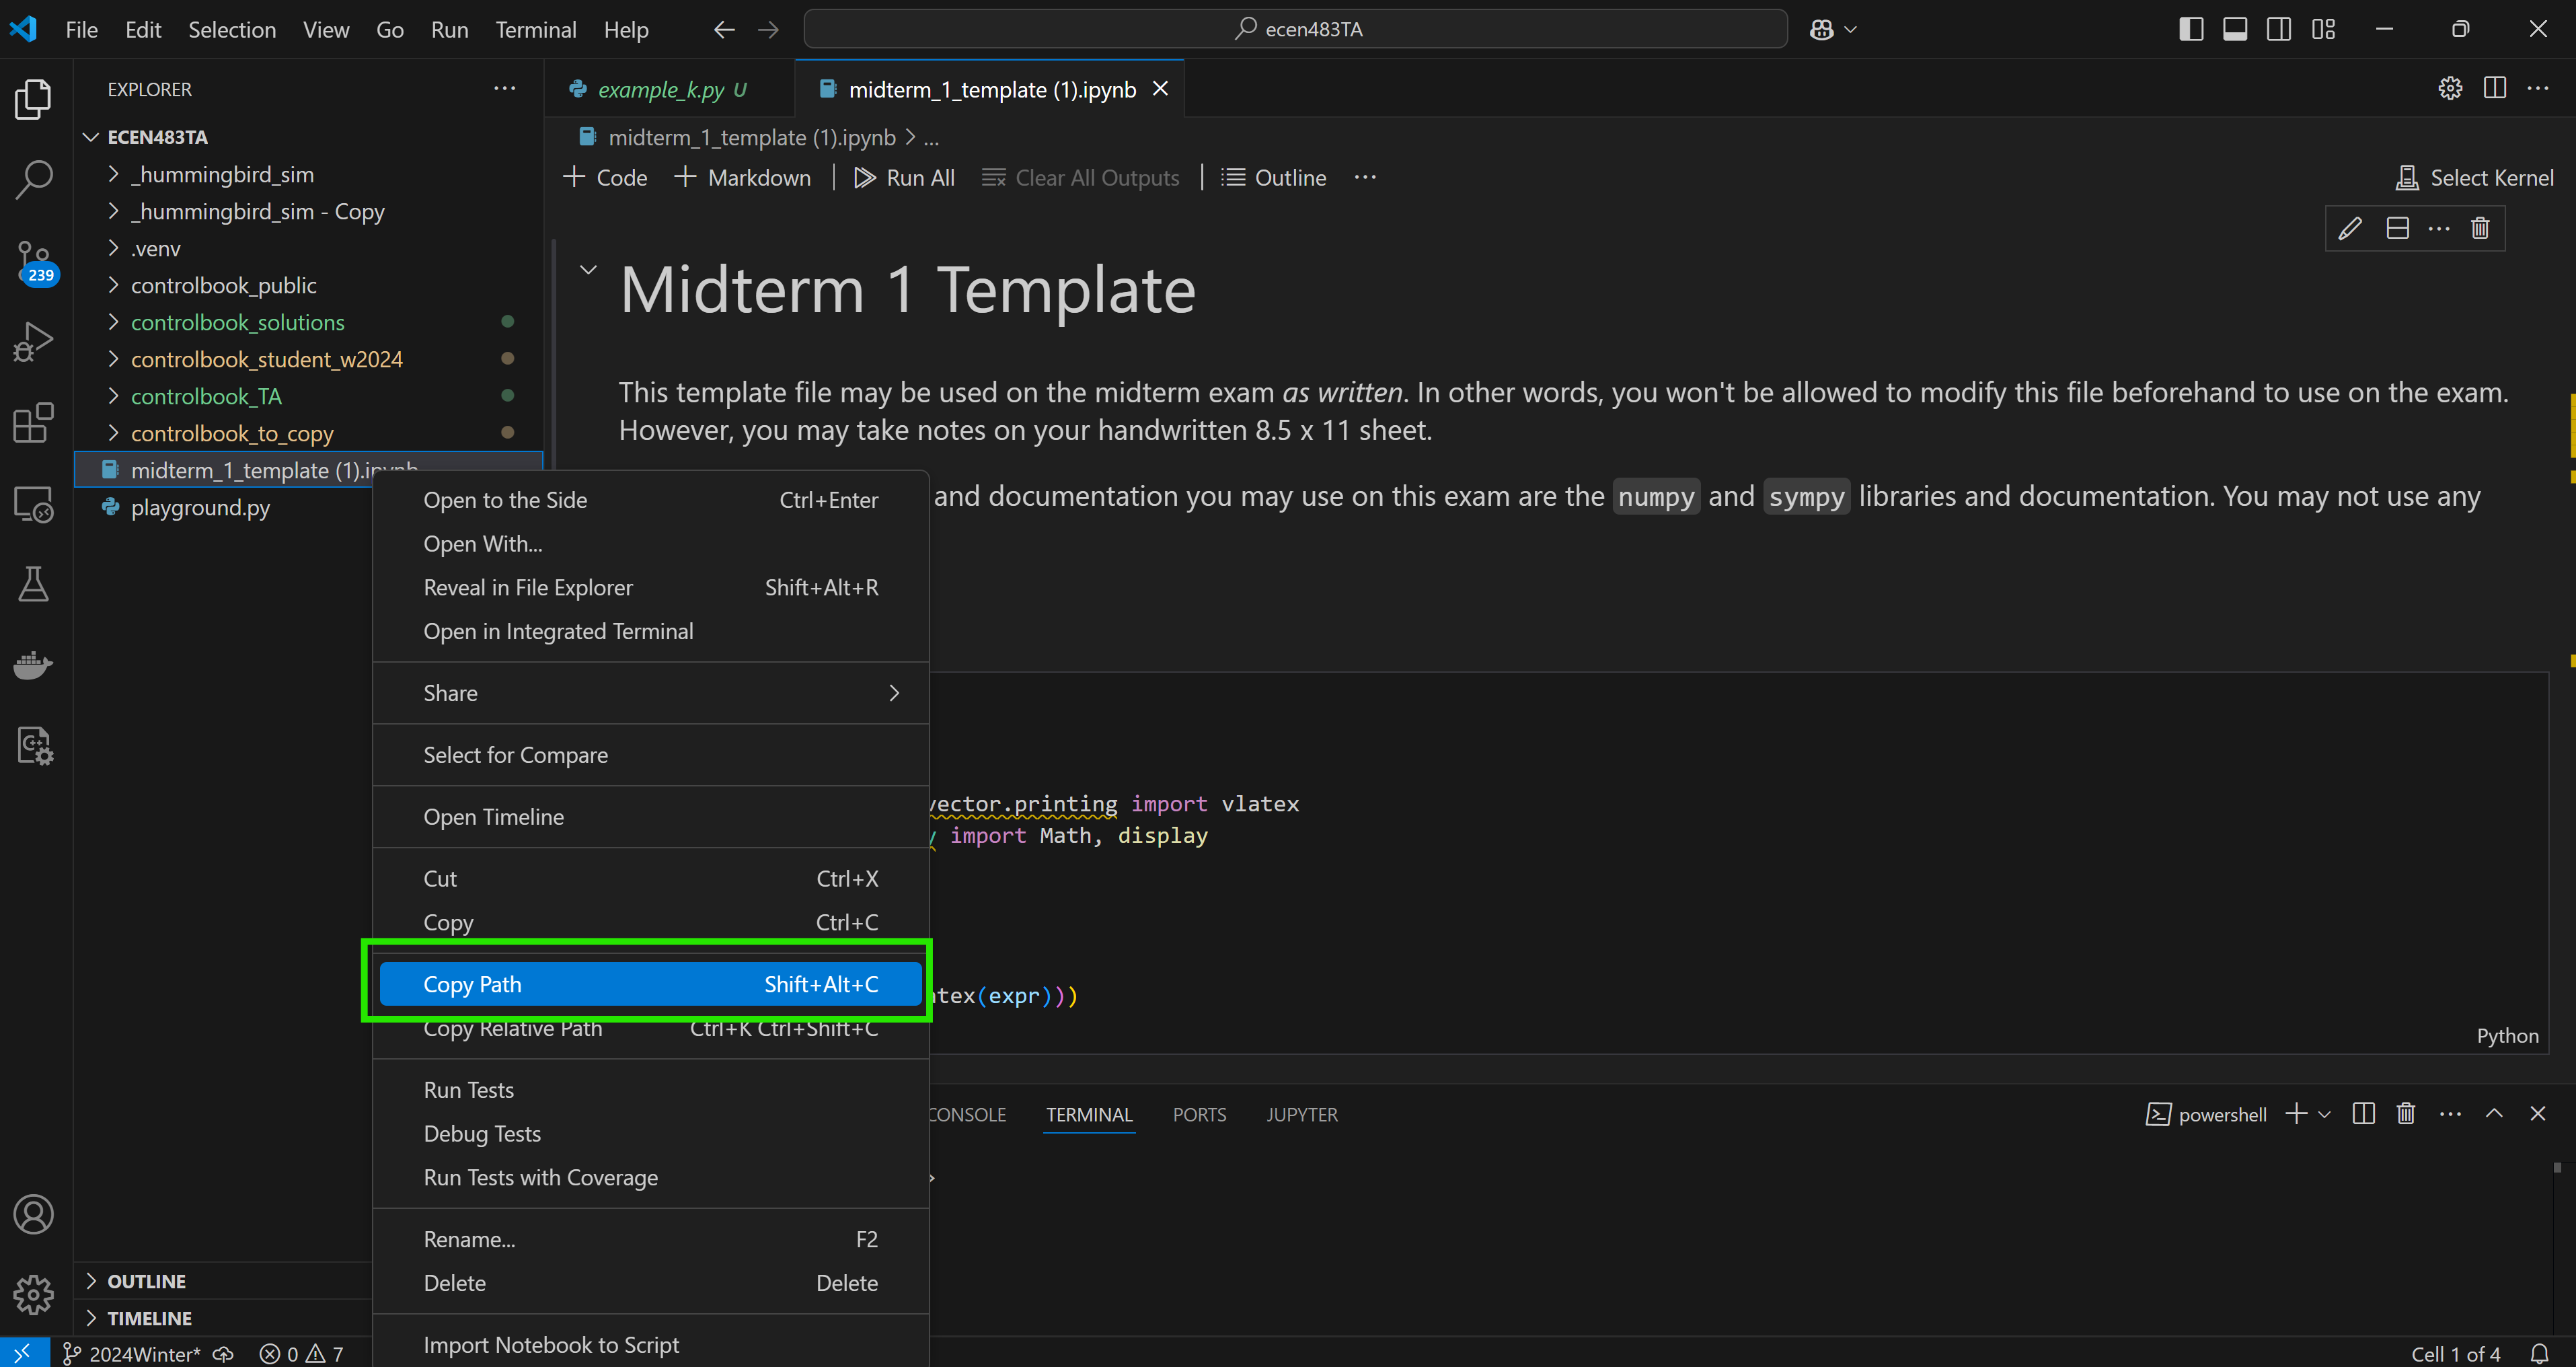
\includegraphics[width=\linewidth]{pic9-copy_path.png} 
    \captionof{How to grab Path with Midterm Template as an example. \footnote{This is different from Relative Path, which grabs the path relative to the project.}}
\end{center}

\begin{center}
    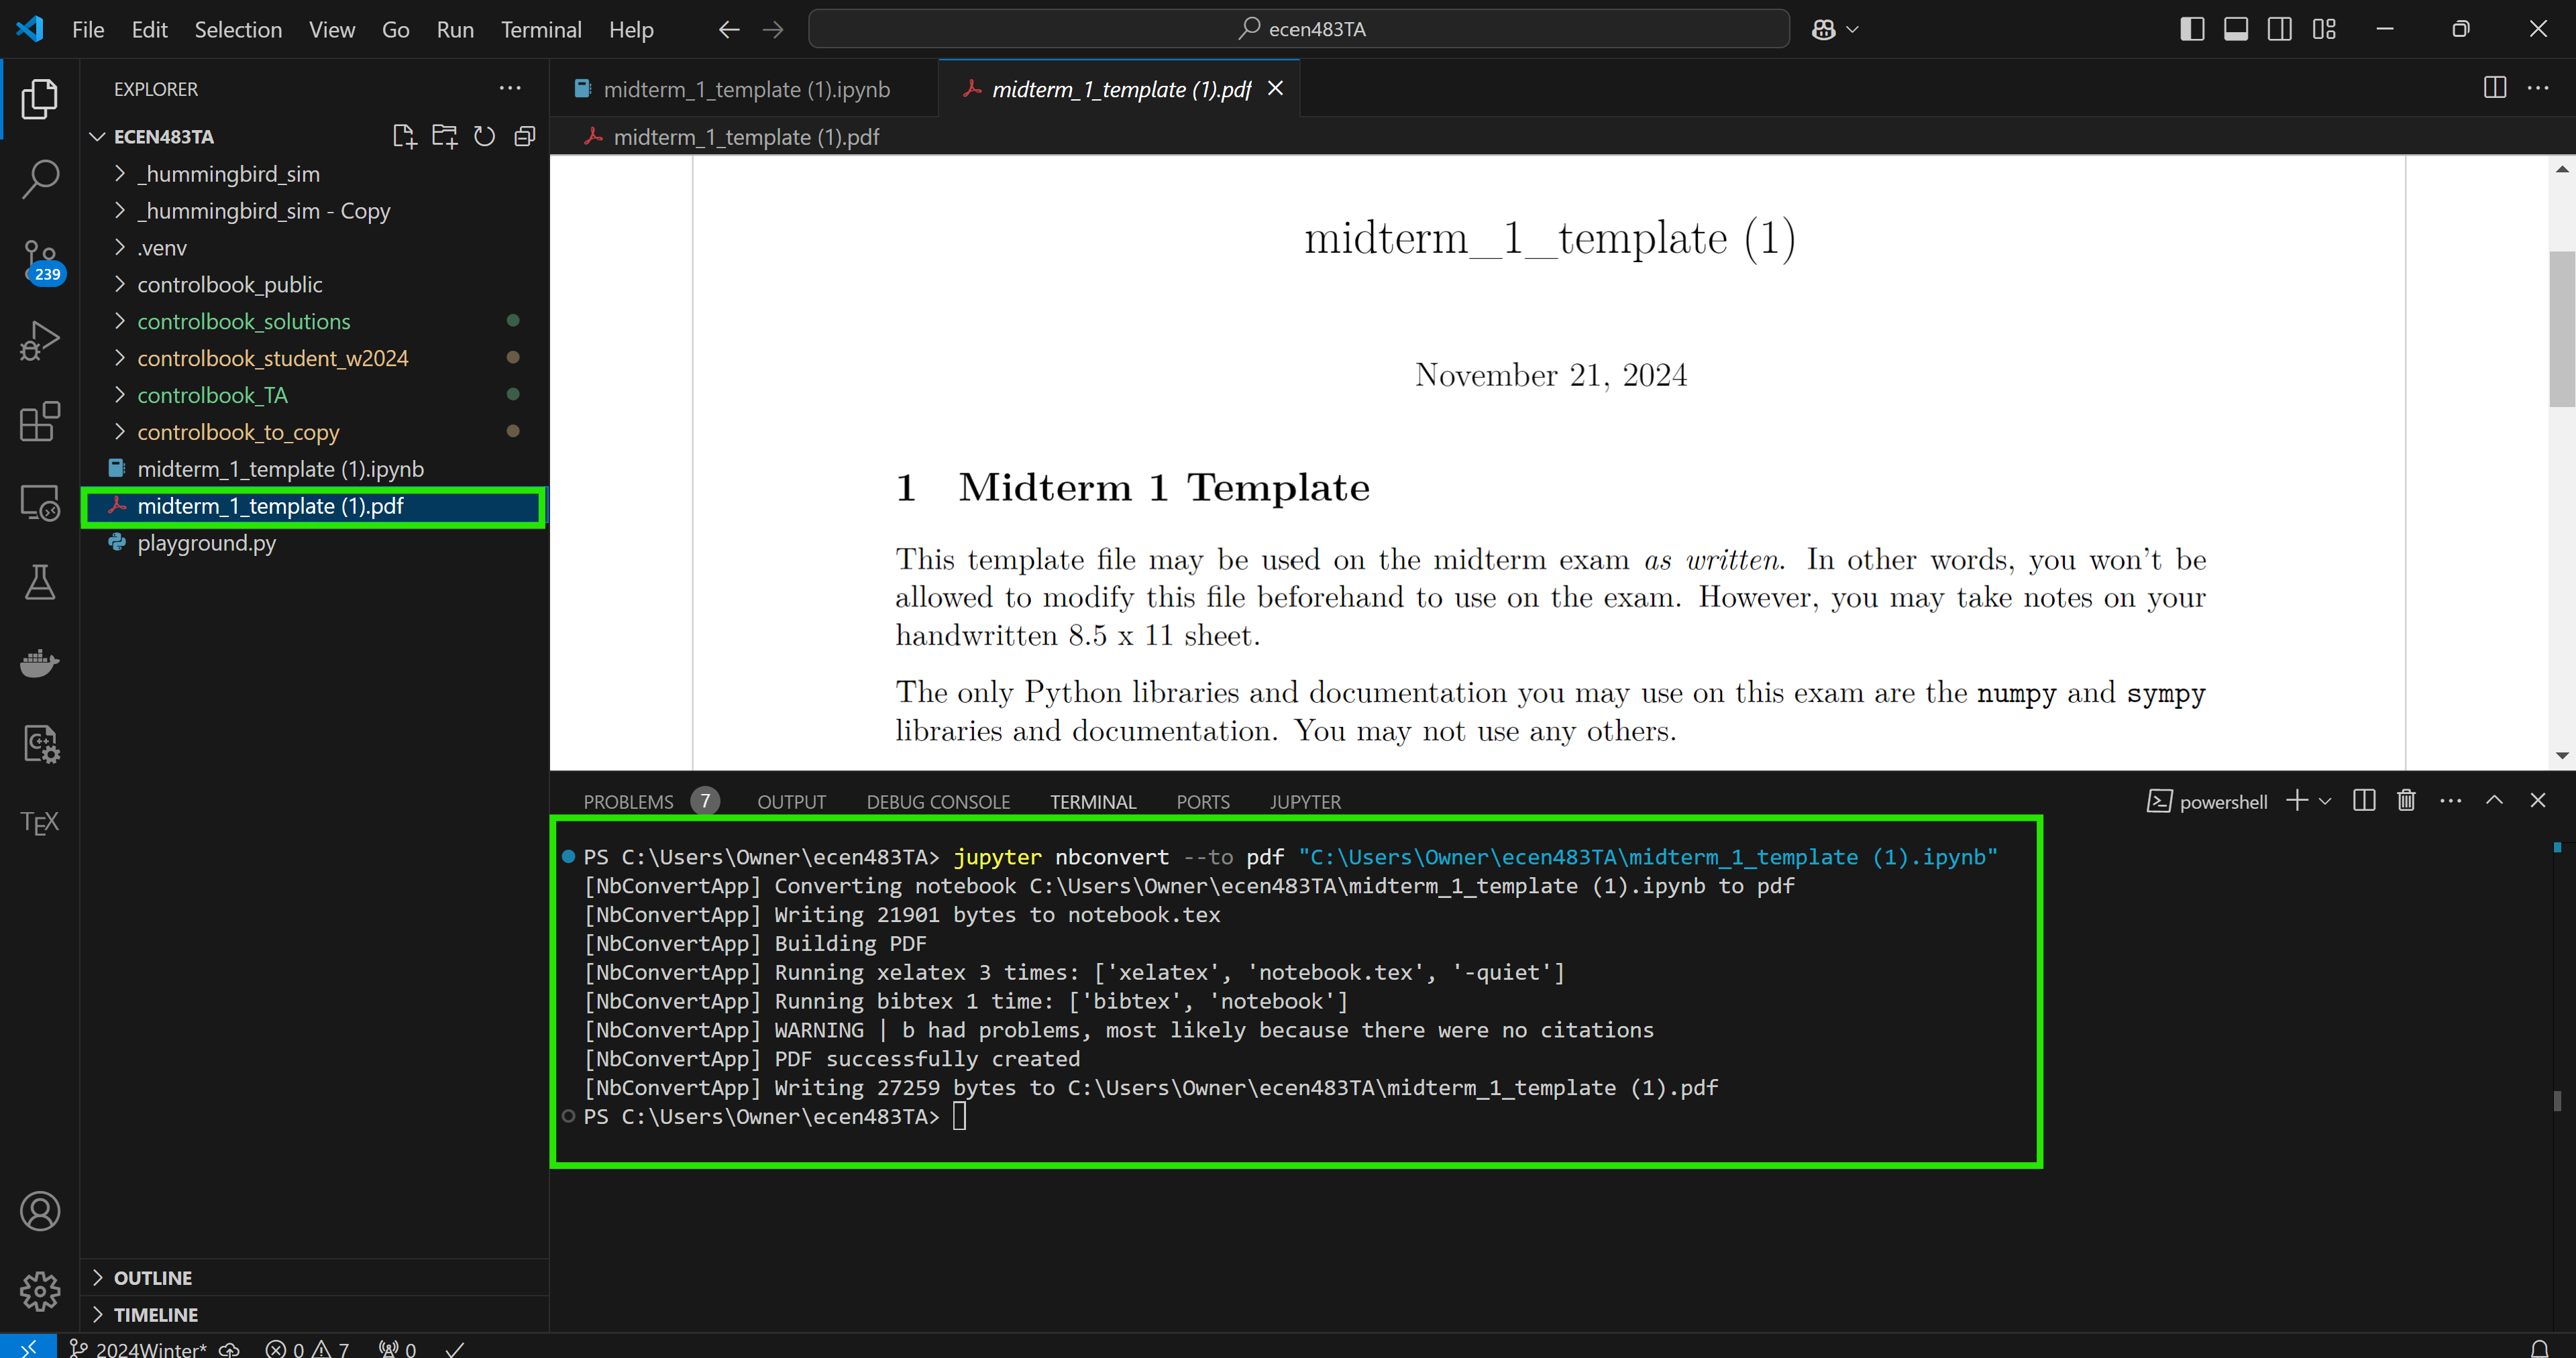
\includegraphics[width=\linewidth]{pic11-output.png} 
    \captionof{Result of converting to notebook with Midterm Template as an example.}
\end{center}

This command will create a PDF file with the same name as the notebook file. If \LaTeX~is not installed or you encounter issues, consider applying the installations below. If those do not allow it to run, consider using one of the alternative methods below the installation instructions below it.

\subsubsection{Installing \TeX~Distributions: TeXLive and MiKTeX}

To convert a Jupyter Notebook directly to PDF using \texttt{nbconvert}, a \TeX~distribution such as TeXLive or MiKTeX is required. Below are steps to install each of these distributions on various operating systems.

\paragraph{Installing TeXLive}
TeXLive is a comprehensive \TeX~distribution available for Linux, macOS, and Windows.

\begin{itemize}
    \item \textbf{Linux}: TeXLive is usually available in the package manager. For instance, on Debian-based systems, run:
    \begin{verbatim}
    sudo apt-get install texlive-full
    \end{verbatim}
    On other Linux distributions, use the equivalent package manager command.
    
    \item \textbf{macOS}: TeXLive can be installed via MacTeX, which includes TeXLive and other useful tools. Download it from \url{https://www.tug.org/mactex/} and follow the installation instructions.
    
    \item \textbf{Windows}: Download the TeXLive installer from \url{https://www.tug.org/texlive/}. Run the installer and follow the on-screen instructions.
\end{itemize}

\paragraph{Installing MiKTeX}
MiKTeX is a lightweight \TeX~distribution, primarily used on Windows but also available for macOS and Linux.

\begin{itemize}
    \item \textbf{Windows}: Download the MiKTeX installer from \url{https://miktex.org/download}. Run the installer and select the default settings for a typical installation.
    
    \item \textbf{macOS and Linux}: MiKTeX also provides installers for macOS and Linux, available on the same website. Download the appropriate installer and follow the installation instructions provided.
\end{itemize}

After installing either TeXLive or MiKTeX, ensure that the \TeX~distribution’s binary directory is added to your system’s PATH, so it is accessible from the command line. Once installed, \texttt{nbconvert} can use \LaTeX~to compile notebooks directly into PDF format.





\subsection{To Python Script to PDF}

Another way to obtain a PDF from a Jupyter Notebook is to first convert the notebook to a Python script. This approach allows for further customization before generating the final PDF.

\begin{enumerate}
    \item Convert the notebook to a Python script using the command line:
    \begin{verbatim}
    jupyter nbconvert --to script notebook.ipynb
    \end{verbatim}
    This command will produce a \texttt{.py} file containing the notebook code and markdown comments.
    
    \item Alternatively, in Visual Studio Code (VSCode), a Jupyter Notebook can be exported as a Python file directly via the graphical interface. Open the notebook in VSCode and select the option to \texttt{Export As Python Script}. 
    % Image can be added here for VSCode GUI
    % \includegraphics[width=\textwidth]{vscode_export.png}

    \item Open the \texttt{.py} file in a text editor and make any adjustments if necessary. Then, convert it to PDF using a tool like \texttt{Pweave} (for formatting Python scripts) or by running the script and saving outputs directly.
\end{enumerate}


\subsection{To HTML to PDF}

If \LaTeX~is not installed, an easy alternative is to convert the notebook to HTML format and print it as a PDF.

\begin{enumerate}
    \item Convert the notebook to HTML:
    \begin{verbatim}
    jupyter nbconvert --to html notebook.ipynb
    \end{verbatim}
    This command will generate an HTML file, which preserves the notebook’s formatting and interactive elements.
    
    \item Open the resulting HTML file in a web browser. From the browser’s print menu, select \texttt{Print to PDF} to save the notebook as a PDF file.
\end{enumerate}

Each of these methods has its benefits depending on the complexity of the notebook and the available software. For example, the HTML-to-PDF route may work best for basic formatting needs, while the \texttt{nbconvert -to pdf} method provides greater fidelity when \LaTeX~is installed.

\section{Editing This Document with Github}

See \href{https://www.zonca.dev/posts/2023-02-02-github-overleaf#:~:text=Create%20a%20new%20repository%20on,this%20repository%20under%20your%20account.}{this link}.



\end{document}
